\documentclass[a4paper,10pt,english]{article}
\usepackage[utf8]{inputenc}
\usepackage[norsk]{babel}
% Standard stuff

\usepackage{amsmath,graphicx,varioref,verbatim,amsfonts,geometry,grffile}
% colors in text
\usepackage[usenames,dvipsnames,svgnames,table]{xcolor}
% Hyper refs
\usepackage[colorlinks]{hyperref}
\usepackage{flafter}
\usepackage{float}
\usepackage{placeins}
\usepackage{fancyvrb}
\usepackage{comment}
\usepackage{csquotes}


% Document formatting
\setlength{\parindent}{0mm}
\setlength{\parskip}{1.5mm}

%Color scheme for listings
\usepackage{textcomp}
\definecolor{listinggray}{gray}{0.9}
\definecolor{lbcolor}{rgb}{0.9,0.9,0.9}

%Listings configuration
\usepackage{listings}
%Hvis du bruker noe annet enn python, endre det her for å få riktig highlighting.
\lstset{
	backgroundcolor=\color{lbcolor},
	tabsize=4,
	rulecolor=,
	language=python,
        basicstyle=\scriptsize,
        upquote=true,
        aboveskip={1.5\baselineskip},
        columns=fixed,
	numbers=left,
        showstringspaces=false,
        extendedchars=true,
        breaklines=true,
        prebreak = \raisebox{0ex}[0ex][0ex]{\ensuremath{\hookleftarrow}},
        frame=single,
        showtabs=false,
        showspaces=false,
        showstringspaces=false,
        identifierstyle=\ttfamily,
        keywordstyle=\color[rgb]{0,0,1},
        commentstyle=\color[rgb]{0.133,0.545,0.133},
        stringstyle=\color[rgb]{0.627,0.126,0.941}
        }
        
\newcounter{subproject}
\renewcommand{\thesubproject}{\alph{subproject}}
\newenvironment{subproj}{
\begin{description}
\item[\refstepcounter{subproject}(\thesubproject)]
}{\end{description}}

%\lstset{inputpath="C:/Users/Jon Andre/Python/Ast2000/Dunno"}
%\graphicspath{{C:/Users/Jon Andre/Python/Ast2000/Dunno/}}
%\numberwithin{equation}{section}


\begin{document}
\title{Solutions to exercise in part 2A}
\author{Jon A Ottesen}
\maketitle
\clearpage


\section*{Usefull fromulas}
\subsection*{Law of constant motion (in one dimention)}
If an object moves a distance $\Delta x$ with constant velocity $v$ in the time interval $\Delta t$, the velocity is given by 
\begin{equation}\label{eq:const_mot}
v=\frac{\Delta x}{\Delta t}
\end{equation}


\subsection*{The Lorentz transformation (in one dimention)}
Assume that we have two coordinate systems: one moving along the x-axis with velocity $v$, and another one at rest. If the coordinates for an event is given by $(x^{\prime},t^{\prime})$ in the moving frame and by $(x,t)$ in the non-moving frame, then we can converte the coordinates between the two frames as follows:

\begin{align}
t&=v\gamma x^{\prime}+\gamma t^{\prime}\\
t&=\gamma x^{\prime}+v\gamma t^{\prime}\\ \nonumber\\
t^{\prime}&=-v\gamma x+\gamma t\\
x^{\prime}&=\gamma x-v\gamma t
\end{align}

Here $\gamma=\frac{1}{\sqrt{1-v^{2}}}$.


\subsection*{Time dilation and length contraction}
Assume that we have two coordinate systems: one moving along the x-axis with velocity $v$, and another one at rest. If the time for an event is given by $\Delta t^{\prime}$ in the moving frame and by $\Delta t$ in the non-moving frame, then we can find the time in one frame given the time in the other as follows:

\begin{equation}\label{eq:time_dila}
\Delta t=\gamma\Delta t^{\prime}
\end{equation}

If we know that the distance between the two events are $\Delta x^{\prime}=L_{0}$ in the moving frame and $\Delta x=L$ in the non-moving frame, then we can find the distance in one frame given the distance in the other as follows:

\begin{equation}\label{eq:len_con}
L=\frac{L_{0}}{\gamma}
\end{equation}

Here $\gamma=\frac{1}{\sqrt{1-v^{2}}}$. Both of these equations can be derived from the Lorenz transformations.

\newpage









\section*{Exercise 2A.1}

\begin{enumerate}

\item Since both of the cylinders are centered around the same axis, cylinder B pass trough cylinder A if it has sufficiently large velocity (assuming that the radius of cylinder B shrinks with velocity along the x-axis).

\item For an observer positioned on cylinder B, cylinder A will from his point of view be moving towards him, while  cylinder B is standing still. Thus the radius of sylinder A will shrink and therefor pass trough cylinder B.

\item The observations made in the earlier tasks shows that whichever cylinder passes through which depends on the referencesystem. Therefor z=z' and y=y' must be true to avoid contradictions.\\

\end{enumerate}









\section*{Exercise 2A.2}

\begin{enumerate}

\item Find answer in MCast

\item Find answer in MCast\\

\item The speed of the spaceship without acceleration is given by the law of constant velocity \ref{eq:const_mot}
\[v=\dfrac{s}{t}\]
In the spaceship frame the roles are changed and it is the planet that has velocity $v=\dfrac{s}{t}$. (The numerical answer can be found in document $\ldots$)

\item (In this case the solution, regardless of the frame of reference, is the same.) The space-time interval is defined as

\begin{equation*}
\Delta s^2=\Delta t^2-\Delta x^2
\end{equation*}

where $\Delta t$ is time difference between event A (spaceship enters the atmosphere) and G (spaceship hits the ground), while $\Delta x$ is the distance between the two events (remember that units of $\Delta t$ and $\Delta x$ must be equal). The spacetime interval becomes

\begin{align*}
\text{(spaceship frame:)} && \Delta (s_{AG}^{\prime})^2&=(\Delta t_{AG}^{\prime})^{2}-0^{2}=\left(t_G^{\prime}-t_A^{\prime}\right)^2\\
\text{(planet frame:)} && \Delta s_{AG}^2&=\Delta t_{AG}^2-\Delta x_{AG}^2=\left(t_G-t_A\right)^2-\dfrac{x_A^2}{c^2}
\end{align*}
where $x_A$ is the distance from the ground to the beginning of the atmosphere.\\ (Remember that the spaceship is always centered at $x=0$ in the rest frame of the spaceship, thus $\Delta x^{\prime}_{AG}=0$. Look up the definition of proper time in the lecture notes.)

\item Invariance of the space-time interval gives us (see pervious task for the other space-time interval)

\begin{align*}
(\Delta s_{AG}^{\prime})^{2}&=\Delta s_{AG}^{2}\\
(\Delta t_{AG}^{\prime})^2&=\Delta t_{AG}^2-\dfrac{\Delta x_{AG}^2}{c^2}
\end{align*}

Equation \ref{eq:const_mot} (definition of constant velocity) gives us $\Delta x_{AG}=\Delta t_{AG}\cdot v$. Thus

\begin{align}
(\Delta t_{AG}^{\prime})^2&=\Delta t_{AG}^2-\Delta t_{AG}^2\dfrac{v}{c^2} \nonumber\\
(\Delta t_{AG}^{\prime})^2&=\Delta t_{AG}^2\left(1-(v/c)^2\right) \nonumber\\
\Delta t_{AG}^{\prime}&=\Delta t_{AG}\sqrt{1-\nu^2}=\dfrac{\Delta t_{AG}}{\gamma}\label{eq:time_dilation}
\end{align}
which can be solved for the desired frame. Be aware that $\nu=v/c$. (The numerical answer can be found in document $\ldots$)

\item We are now looking at muons that are produced high up in the atmosphere, traveling at velocity $v=0.999c$. We want to find the time a muon would use to arrive at the surface of the earth.\\
Assuming the muon has constant velocity, equation \ref{eq:const_mot} gives us

\begin{equation*}
\Delta t_{AG}=\dfrac{\Delta x_{AG}}{v}=\dfrac{15km}{0.999c}\approx5.005\cdot 10^{-5}\,s.
\end{equation*}

Hence the muon uses approximentely $50\,\mu s$ to reach the ground (in the planet frame).


\item Since \[50\,\mu s=\Delta t_{AG}>\Delta t_{\text{Muon}}=2\,\mu s,\] where $\Delta t_{\text{Muon}}$ is the mean lifetime of a muon, most muons will never reach the surface of the earth (when we do not take into account relativistic effects).

\item Thinking of the muon as the spaceship from above, we see that this situation is equivalent with the one above. In other words, solving task 1-5 symbolically, we find exactly the expression we want. Hence equation \ref{eq:time_dilation} (which is the equation for time dilation) gives us

\begin{equation*}
t^{\prime}=\dfrac{t}{\gamma}=5\cdot 10^{-5}\sqrt{1-0.999^{2}}\approx2.2\,\mu s
\end{equation*}

Thus a large number of muons will be able to reach earth when relativistic effects are taken into account.

\end{enumerate}









\section*{Exercise 2A.3}

\begin{enumerate}

\item \textbf{For both frames:}

\begin{enumerate}

\item Let event Y be the emission of the yellow light, and event B be the emission of the blue light. The time and position for both events should be found in MCast. Here we will only use symbols. \textbf{Remember that you should know all the values in your own frame of referance.}

\begin{table}[H]
  \begin{center}
    \begin{tabular}{| l | l | l | }
   	\hline
	 Time or position & Event Y & Event B \\ \hline
	 $t$ & $t_Y$ & $t_B$ \\ \hline
	 $x$ & $x_Y$ & $x_B$ \\ \hline
	 $t^{\prime}$ & $t_Y^{\prime}$ & $t_B^{\prime}$ \\ \hline
	 $x^{\prime}$ & $x_Y^{\prime}=0$ & $x_B^{\prime}=0$ \\ \hline
	\end{tabular}
    \caption{The different times and positions for task 2A.3 1. (You should look up these in MCast.)}
    \label{tabel:1}
  \end{center}
\end{table}
\FloatBarrier

\item The time intervals is therefore $\Delta t_{YB}=t_{Y}-t_{B}$ and $\Delta t_{YB}^{\prime}=t_Y^{\prime}-t_B^{\prime}$ (put in the numbers you found in MCast for numerical answer. Correct answers are given in document $\ldots$).

\end{enumerate}

\item See next task.
\item (frames are specified when needed below)

\begin{enumerate}

\item
\underline{\bf{Spaceship frame:}} The lights are emitted from the spaceship. Therefore, since the spaceship is moving with a velocity $v$, the positions of the lights (in the planet frame) are

\begin{align*}
x_Y=v\cdot t_Y&\\
x_B=v\cdot t_B
\end{align*} 

\underline{\bf{Planet frame:}} The lights are emitted from the spaceship. Therefore, since the spaceship always is centered at the origin in the spaceship frame, the positions of the lights (in the spaceship frame) are

\begin{align*}
x^{\prime}_Y=0&\\
x^{\prime}_B=0
\end{align*} 

\item The space-time interval for the \underline{planet frame} is

\begin{align*}
\Delta s_{YB}^2&=\Delta t_{YB}^2-\Delta x_{YB}^2=\left(t_B-t_Y\right)^2-\left(x_B-x_Y\right)^2\\&=\left(t_B-t_Y\right)^2-\left(v\cdot t_B-v\cdot t_Y\right)^2=\left(t_B-t_Y\right)^2-v^2\left(t_B-t_Y\right)^2\\&=\left(t_B-t_Y\right)^2(1-v^2)=\Delta t_{YB}^2(1-v^2)\\&=\frac{\Delta t_{YB}^2}{\gamma^2}
\end{align*}

The space-time interval for the \underline{spaceship frame} is

\begin{align*}
(\Delta s_{YB}^{\prime})^2&=(\Delta t_{YB}^{\prime})^2-(\Delta x_{YB}^{\prime})^2\\&=\left(t_B^{\prime}-t_Y^{\prime}\right)^2-\left(x_B^{\prime}-x_Y^{\prime}\right)^2\\&=\left(t_B^{\prime}-t_Y^{\prime}\right)^2-0^2\\&=(\Delta t_{YB}^{\prime})^2=\Delta \tau^2
\end{align*}

\item Using invarianse of the space-time interval we find that

\begin{align*}
(\Delta s_{YB}^{\prime})^2&=\Delta s_{YB}^2\\
(\Delta t_{YB}^{\prime})^2&=\frac{\Delta t_{YB}^2}{\gamma^2}\\
\Delta t_{YB}^{\prime}&=\frac{\Delta t_{YB}}{\gamma}
\end{align*}

Which is exactly the expression for time dilation \ref{eq:time_dila}. (The numerical answer can be found in document $\ldots$)

\end{enumerate}

\item From length contraction we know that $L=L_0/\gamma$, hence the length between the two lights should be largest in the rest frame. You should therefore observe a larger distance in the planet frame.   

\end{enumerate}









\section*{Exercise 2A.4}
\textbf{Del inn i parts\\Hva ønsker vi å gjøre i denne oppgaven? Flere av spørsmålene gjøres bare på måfå. Gjør spørsmålene mer som part 2 2.\\Si hvilken vei de beveger seg (mot venstre eller høyre?)\\part 1 3. samme spørsmål stilles to ganger.\\I part1 7. dropp siste setningen om å finne L (skaper bare forvirring). Vurder å bruke $L_{0}$ isteden for $L^{\prime}$ for å være konsekvent. Kanskje si noe om å finne tall i MCast for å regne ut $L^{\prime}$ og $t_{C}^{\prime}=t_{D}^{\prime}$.\\ I part 1 8. si at man skal bruke hastighet til å beskrive eventene også.\\ Part 1 10. litt rar setning.\\Part 1 11. funksjon i hviken frame?\\Part 1 12. minn dem på at de har funnet et uttrykk for $t_{D}$\\Part 2 1. omformuler beam 1. Er ikke mye av dette allerede gjort?\\Part 2 2. kall $t_{X}$ for $t_{M}$.\\Part 2 3. Hvorfor finne $t_{x}$ hvis du ikke skal bruke den?\\Part 2 8. det må komme tydligere frem at $L=L^{\prime}$ (vet ikke om lengdekontraksjon).\\Part 2 9. minn på at vi ikke tok hensyn til lengdekontraksjon.\\Part 1 slå sammen 2 og 3.\\Part 1 7. slå sammen 7 og deler av 8 og be om ``make an event table where you put in numbers for the values in the spaceship frame'' eller noe liknende.\\Part 2 1. har allerede funnet posisjon til venstre/høyre laser. Skal de gjøre det igjen?}
\subsection*{Part 1}

We are studying two spaceships moving from left to right with velocity $v$ in the planet frame (in the spaceship frame, the planet is moving from right to left). An observer M, right in between the two spaceships, also move from left to right with velocity $v$, thus it is in the same frame as the spaceships.
\\
We let $(x,t)$ and $(x^{\prime},t^{\prime})$ denote the planet and spaceship frame respectively. In this exercise we are studying the four following events:
\begin{enumerate} %\begin{itemize}
\item Event A is when the left spaceship fires a deadly laser. This happens at $t_{A}=t_{A}^{\prime}=0$ and $x_{A}=x_{A}^{\prime}=0$.
\item Event B is when the right spaceship fires a deadly laser. This happens simultaneously as event A in the spaceship frame.
\item Event C is when the left spaceship explodes. This happens when the laser from the right spaceship hits the left spaceship.
\item Event D is when the right spaceship explodes. This happens when the laser from the left spaceship hits the right spaceship.
\end{enumerate} %\end{itemize}

In the first tasks we will pretend that the only thing we know about the theory of relativity is that the velocity of light is equal for all observers.

\begin{enumerate}
\item We want to show that the laser beams cross at observer M's position. Since we know that the velocity of light is equal for all observers, we know that light travels through space with velocity $c=1$ (remember that velocity is unitless when working with relativity) in the spaceship frame. Thus the left laser travels with velocity $v=c=1$ and the right laser travels with velocity $v=-c=-1$. The spaceships do not with respect to the lasers in the spaceship frame, hence (since observer M is in the same frame of referance as the spaceships) observer M will always stay in the middle. Assuming that the distance between the two spaceships is $L^{\prime}$, the position of the lasers in the spaceship frame are (remember the definition of constant velocity \ref{eq:const_mot})
\begin{align*}
x_{\text{Left laser}}=c\cdot t=t &&\text{and}&& x_{\text{Right laser}}=L^{\prime}-c\cdot t=L^{\prime}-t
\end{align*}
The lasers will meet when $x_{\text{Left laser}}=x_{\text{Right laser}}$. Solving this equation with respect to time we find
\begin{align*}
x_{\text{Left laser}}&=x_{\text{Right laser}}\\
t&=L^{\prime}-t\\
t&=L^{\prime}/2
\end{align*}
Inserting this time into the position for one of the lasers (or remebering that since time and position are measured in the same units) we get 
\[x_{\text{Left laser}}=L^{\prime}/2=x_{\text{Right laser}}\]
Finally, since observer M's position is right in between the two spaceships, we must have 
\[x_{M}=x_{\text{Left laser}}=x_{\text{Right laser}}=L^{\prime}/2\]
In other words, the lasers will cross at observer M's position.

\item We want to explain why event A and B could not have been simultaneous in the planet frame. To explain this we need to explain why the lasers cross at the position of observer M in the planet frame too. 
\\
The first axiom of relativity tells us that if an event occures in one frame of referance, it must occure in every frame of referance (this must be valid even though we do not know anything about relativity, if not, we can create paradoxes as explained in the lecture note). Since the lasers crossing at observer M can be regarded as an event, this must happen in every frame of referance, including the planet frame. 
\\
We can now explain why the two events cannot be simultaneous in the planet frame. Observer M moves with the spaceships at a velocity $v$, the left lasers move with velocity $c=1$ and the right lasers move with velocity $-c=-1$ in the planet frame. This means that after a time $\Delta t$ the left laser reaches the point where observer M was when it was fired, but observer M has now moved a distance $v\Delta t$ further. For the right laser we have an opposite case: before it reaches the point where observer M was when it was fired, observer M will have moved enough to reach the laser.
\\
In other words, the left laser must travel a greater distance then the right laser. Since they are supposed to meet at M in all frames of referance and the two lasers have the same absolute velocity, the left laser must be fired first to give it enough time to reach observer M.
\textbf{Her er 2 og 3 slått sammen. Altså er 3=4, 5=6, osv.}

\item We now move on to the explosions. We understand that these have to be simultaneous in the spaceship frame and we want to explain why they cannot be simultaneous in the planet frame.
\\
In the pervious task we defined event A to be the origin of our spacetime coordinate system, but this need not be the origin. We now redefine the origin to be at the explosion of the left spaceship (we will only redefine the origin for this task to see the conclsion easier, but it is not needed and we will go back to our original definition of the origin after this task). Some of the light created from the explosion will travel towards M. This is true for both spaceships. Since the only thing that has changed from the pervious tasks is where the origin is and that we are observing light insted of a deadly laser, we have an identical case and can now think of event A and B as the explosion of the left and right spaceship respectively. Yet again the light from both explosion will cross at observer M's position and by our above deduction, we know that the explosions cannot be silutaneous in the planet frame (unless the velocity of the spaceships are $v=0$).

\item It is not difficult to understand which explosion occures first in the planet frame now. Thinking of the light from the explosions as the lasers from event A and B, the above deduction tells us that the left spaceship must have exploded first.

\item The order of the events in the planet frame must be A, B, C and D:
\\
We know that the left laser has a longer way to travel to reach observer M then the right laser, hence event A must occure first to give the left laser enough time to reach observer M simultaneos as the right laser. Since the two lasers are supposed to meet at observer M's position (before any of the spaceships explode), we know that event B must happen next.
\\
We have explained that the light from the explosion must reach M simultaneously in the spaceship frame, thus event C (the left spaceship exploding) must occure next since the light from the explosion has a larger distance to travel to reach M. Finally event D happens last so that the light from both explosion meet at observer M.
\\
\textbf{Kan kanskje inkludere bilde(?)}
\end{enumerate}

\begin{enumerate}
\setcounter{enumi}{5}

\item We will solve task 6 and 7 in one go.
\item Let $(x,t)$ and $(x^{\prime},t^{\prime})$ denote the space-time coordinates in the planet and spaceship frame respectively. We are going to set up an event table for the four events A, B, C and D.
\\ \\
We begin with some info. You should know the value of all the spaceship variables, that is, all marked variables should be known (look these up in MCast). We let $L$ and $L^{\prime}$ be the distance between the spaceships in the planet and spaceship frame respectively. We are specifically asked to measure both time and distance in kilometers [$km$]. This means that when you find times in MCast, you will need to multiply them by the speed of light \[\frac{t_{m}}{t_{s}}=c,\] where $t_{m}$ is time measured in meters and $t_{s}$ is time measured in seconds. We are now ready to solve the task.
\\ 
\begin{enumerate} %\begin{itemize}
\item We are told that event A happens at $t_{A}=t_{A}^{\prime}=0$ and $x_{A}=x_{A}^{\prime}=0$. Next we are told that event A and B are simultaneous in the spaceship frame, and we know that the distance between the the two spaceships are $L$ and $L^{\prime}$ in the planet and spaceship frame respectively, therefore giving $t_{B}^{\prime}=t^{\prime}_{A}$ and $x_{B}^{\prime}=L^{\prime}$.

\item Since both spaceships and observer M is at rest in the spaceship frame we must have $x_{C}^{\prime}=0$ and $x^{\prime}_{D}=L^{\prime}$. Because event C and D are simultaneous in the spaceship frame, $t^{\prime}_{D}=t^{\prime}_{C}$.

\item We are only missing an expression for the position of event B, C and D in the planet frame. The pervious tasks show that non of these events are simultaneous in the planet frame, but we know that the spaceships travel with the same velocity $v$ and are therefore always a distance $L$ apart ($L$ will be unknown for now). Since the events happen after times $t_{B}$, $t_{C}$ and $t_{D}$ we get (remember that the initial position of the spaceships are $0$ and $L$, and they will have moved a distance $v\cdot t$ after a time $t$) 
\begin{align*}
x_{B}=L+vt_{B} && x_{C}=vt_{C} && x_{D}=L+vt_{D}
\end{align*}
\end{enumerate} %\end{itemize}
We should aslo note that since time and distance is measured in the same units, the definition of constant velocity \ref{eq:const_mot} for light tells us that $\Delta x=v\cdot\Delta t=\overbrace{c}^{=1}\cdot\Delta t=\Delta t$. This means that $L^{\prime}=t_{C}^{\prime}$ because the laser, which travel with velocity $c$, use $t_{C}^{\prime}$ time to reach the right spaceship. Now it is just a matter of putting the expressions in the table.

\begin{table}[H]
  \begin{center}
    \begin{tabular}{| l | l | l | l | l |}
   	\hline
	 Time or position & Event A & Event B & Event C & Event D\\ \hline
	 $t$ & $t_{A}=0$ & $t_{B}$ & $t_{C}$ & $t_{D}$\\ \hline
	 $t^{\prime}$ & $t^{\prime}_{A}=0$ & $t_{B}^{\prime}=t^{\prime}_{A}=0$ & $t_{C}^{\prime}$ & $t^{\prime}_{D}=t^{\prime}_{C}$\\ \hline
	 $x$ & $x_{A}=0$ & $x_{B}=L+vt_{B}$ & $x_{C}=vt_{C}$ & $x_{D}=L+vt_{D}$\\ \hline
	 $x^{\prime}$ & $x^{\prime}_{A}=0$ & $x_{B}^{\prime}=L^{\prime}=t_{C}^{\prime}$ & $x_{C}^{\prime}=0$ & $x^{\prime}_{D}=L^{\prime}=t_{C}^{\prime}$\\ \hline
	\end{tabular}
    \caption{Times and positions for events A, B, C and D. You should know the values of all variables in the spaceship frame. Look these up in MCast.}
    \label{tabel:ex_2A_4}
  \end{center}
\end{table}
\FloatBarrier


\item Let $x_{Lb}$ denote the position of the left laser beam. Remember that the left laser has velocity $c=1$ (in the positive direction).
\\
Since event A occures at $x_{A}=0$ and $t_{A}=0$, the left lasers position must be 
\begin{equation}\label{eq:left_laser}x_{Lb}=c\cdot t=t\end{equation}
We know that when $t=t_{D}$ the left laser and right spaceship collide, but this means that their position must be equal.
\begin{align*}
x_{Lb}&=x_{D}\\
t_{D}&=L+vt_{D}\\
t_{D}&=\frac{L}{1-v}
\end{align*}

Inserting the new expression for $t_{D}$ into the position of event D we find

\begin{equation*}
x_{D}=L+vt_{D}=L+v\frac{L}{1-v}=L\left(\frac{1-v}{1-v}+\frac{v}{1-v}\right)=\frac{L}{1-v}
\end{equation*}

\item We now want to find a new expression for the time $t_{C}$. This can be done using invariance of the space-time interval.

\begin{align*}
\left(\Delta s_{AC}^{\prime}\right)^{2}&=\Delta s_{AC}^{2}\\
\left(\Delta t_{AC}^{\prime}\right)^{2}-\left(\Delta x_{AC}^{\prime}\right)^{2}&=\Delta t_{AC}^{2}-\Delta x_{AC}^{2}\\
\left(t_{C}^{\prime}-\overbrace{t_{A}^{\prime}}^{=0}\right)^{2}-\left(\overbrace{x_{C}^{\prime}}^{=0}-\overbrace{x_{A}^{\prime}}^{=0}\right)^{2}&=\left(t_{C}-\overbrace{t_{A}}^{=0}\right)^{2}-\left(x_{C}-\overbrace{x_{A}}^{=0}\right)^{2}\\
\left(t_{C}^{\prime}\right)^{2}&=t_{C}^{2}-x_{C}^{2}=t_{C}^{2}-(vt_{C})^{2}=(1-v^{2})t_{C}^{2}=\frac{t_{C}^{2}}{\gamma^{2}}\\
t_{C}&=\gamma t_{C}^{\prime}
\end{align*}

This is as expected the formula for time dilation. Inserting this into the position $x_{C}$ we find

\begin{equation*}
x_{C}=vt_{C}=v\gamma t_{C}^{\prime}
\end{equation*}

You should recognize this from the Lorentz transformation $x=\gamma x^{\prime}+v\gamma t^{\prime}$ (remember that $x_{C}=0$, so $\gamma x_{C}^{\prime}=\gamma\cdot0=0$).


\item Let $x_{Rb}$ denote the position of the right laser beam. Remember that the right laser has velocity $-c=-1$. 
\\
Event B occures at $x_{B}=L+vt_{B}$ at some time $t_{B}$. After event B the right laser travels to the left, thus after a time $t$ the position for the laser is given by 
\begin{equation}\label{eq:right_laser}x_{Rb}=L+vt_{B}-(t-t_{B})=L+(v+1)t_{B}-t\end{equation}
The reason for $t-t_{B}$ is so that when $t=t_{B}$ the laser will be at event B. Since the laser moves in the negative direction, the distance it has traveled after it left the right spaceship is $-c(t-t_{B})=-(t-t_{B})$.
\\
We know that when $t=t_{C}$ the right laser and left spaceship collide, but this means that their position must be equal. Since we have already found an expression for $t_{C}$ and $x_{Rb}$ contains the unknown time $t_{B}$, we can solve for the time $t_{B}$.

\begin{align*}
x_{Rb}&=x_{C}\\
L+(v+1)t_{B}-t_{C}&=v\gamma t_{C}^{\prime}\\
L+(v+1)t_{B}-\gamma t_{C}^{\prime}&=v\gamma t_{C}^{\prime}\\
(v+1)t_{B}&=(v+1)\gamma t_{C}^{\prime}-L\\
t_{B}&=\gamma t_{C}^{\prime}-\frac{L}{v+1}
\end{align*}

We can now find the position $x_{B}$.
\begin{equation*}
x_{B}=L+vt_{B}=L+v\left(\gamma t_{C}^{\prime}-\frac{L}{v+1}\right)=v\gamma t_{C}^{\prime}+L\left(\frac{v+1}{v+1}-\frac{v}{v+1}\right)=v\gamma t_{C}^{\prime}+\frac{L}{v+1}
\end{equation*}

\item The only unknown variable that remains is $L$. We will use invariance of the space-time interval between event B and D to find a value for this last variable.

\begin{align}\label{eq:unfiniched_interval}
\left(\Delta s_{BD}^{\prime}\right)^{2}&=\Delta s_{BD}^{2} \nonumber\\
\left(\Delta t_{BD}^{\prime}\right)^{2}-\left(\Delta x_{BD}^{\prime}\right)^{2}&=\Delta t_{BD}^{2}-\Delta x_{BD}^{2} \nonumber\\
\left(\overbrace{t_{D}^{\prime}}^{=t_{C}^{\prime}}-\overbrace{t_{B}^{\prime}}^{=0}\right)^{2}-\left(\overbrace{x_{D}^{\prime}}^{=L^{\prime}}-\overbrace{x_{B}^{\prime}}^{=L^{\prime}}\right)^{2}&=\left(t_{D}-t_{B}\right)^{2}-\left(x_{D}-x_{B}\right)^{2} \nonumber\\
\left(t_{C}^{\prime}\right)^{2}-0^{2}&=\left(t_{D}-t_{B}\right)^{2}-\left(x_{D}-x_{B}\right)^{2}
\end{align}

Before we do any more calculations, lets take a closer look at $\left(t_{D}-t_{B}\right)$ and $\left(x_{D}-x_{B}\right)$.

\begin{equation*}
t_{D}-t_{B}=\frac{L}{1-v}-\left(\gamma t_{C}^{\prime}-\frac{L}{v+1}\right)=L\left(\frac{v+1}{(1-v)(v+1)}+\frac{1-v}{(v+1)(1-v)}\right)-\gamma t_{C}^{\prime}=\frac{2L}{1-v^{2}}-\gamma t_{C}^{\prime}
\end{equation*}

\begin{equation*}
x_{D}-x_{B}=\frac{L}{1-v}-\left(v\gamma t_{C}^{\prime}+\frac{L}{v+1}\right)=L\left(\frac{v+1}{(1-v)(v+1)}-\frac{1-v}{(v+1)(1-v)}\right)-v\gamma t_{C}^{\prime}=\frac{2vL}{1-v^{2}}-v\gamma t_{C}^{\prime}=v\Delta t_{BD}
\end{equation*}

We see that $\Delta x_{BD}=v\Delta t_{BD}$. We can now solve equation \ref{eq:unfiniched_interval} easily.

\begin{align*}
\left(\Delta s_{BD}^{\prime}\right)^{2}&=\Delta s_{BD}^{2}\\
\left(t_{C}^{\prime}\right)^{2}&=\left(t_{D}-t_{B}\right)^{2}-\left(x_{D}-x_{B}\right)^{2}=\left(t_{D}-t_{B}\right)^{2}-v^{2}\left(t_{D}-t_{B}\right)^{2}\\
\left(t_{C}^{\prime}\right)^{2}&=\left(t_{D}-t_{B}\right)^{2}\left(1-v^{2}\right)=\left(\frac{2L}{1-v^{2}}-\gamma t_{C}^{\prime}\right)^{2}\frac{1}{\gamma^{2}}\\
\gamma t_{C}^{\prime}&=\gamma^{2}2L-\gamma t_{C}^{\prime}\\
t_{C}^{\prime}&=\gamma L\\
L&=\frac{t_{C}^{\prime}}{\gamma}=\frac{L^{\prime}}{\gamma}
\end{align*}

As expected, we found the formula for length contraction.

\end{enumerate}

\subsection*{Part 2}
Assuming we do not know anything about relativity again, we want to see if we can deduce the formula for time dilation.

\begin{enumerate}
\item We begin by setting up functions for the positions of the spaceships, observer M and the laser beams. We have already found the position of the two lasers (see equation \ref{eq:left_laser} and \ref{eq:right_laser}) and can therefore focus the spaceships and obeserver M.
\\
We know that they all move with velocity $v$ in positive direction and that their initial positions are $x=0$ (left spaceship), $x=L/2$ (observer M) and $x=L$ (right spaceship). It is now easy to find their positions using the definition of constant velocity \ref{eq:const_mot}.

\begin{align*}
\text{Left spaceship:}& &&& x_{V}&=vt && \text{Left laser:}& && x_{\text{Beam 1}}&=x_{Lb}=t\\
\text{Right spaceship:}& &&& x_{R}&=L+vt && \text{Right laser:}& && x_{\text{Beam 2}}&=x_{Rb}=L+(v+1)t_{B}-t\\
\text{Observer M:}& &&& x_{M}&=L/2+vt
\end{align*}

\item We will now let $t_{X}$ be the time when the two lasers cross at observer M's position. This means that when $t=t_{X}$ the position of observer M and the left laser will be equal (you can find other expressions looking at $x_{M}=x_{\text{Beam 2}}$ and $x_{\text{Beam 1}}=x_{\text{Beam 2}}$, but to find the expression we want, we need to look at the following case).

\begin{align*}
x_{M}&=x_{\text{Beam 1}}\\
L/2+vt_{X}&=t_{X}\\
t_{X}(1-v)&=L/2\\
t_{X}&=\frac{L/2}{1-v}
\end{align*}

\item We now want to find an expression for $t_{B}$. Since the function for the right laser contains $t_{B}$ and we know that when $t=t_{X}$ the right laser's and observer M's position are equal, we find

\begin{align*}
x_{M}&=x_{\text{Beam 2}}\\
L/2+vt_{X}&=L+(v+1)t_{B}-t_{X}\\
(v+1)t_{X}&=L/2+(v+1)t_{B}\\
t_{B}&=t_{X}-\frac{L/2}{v+1}
\end{align*}

\item We can now find the time $t_{C}$ when the left spaceship explodes since the position of the right laser must be equal to the left spaceship at this time.

\begin{align*}
x_{V}&=x_{\text{Beam 2}}\\
vt_{C}&=L+(v+1)t_{B}-t_{C}\\
(v+1)t_{C}&=L+(v+1)\left(t_{X}-\frac{L/2}{v+1}\right)\\
t_{C}&=\frac{L}{v+1}+t_{X}-\frac{L/2}{v+1}\\
t_{C}&=t_{X}+\frac{L/2}{v+1}
\end{align*}

\item We shall now find an expression for the position of the light from the explosion of the left spaceship. We know that the explosion happens at $x=vt_{C}$ (the position of the spaceship when the laser hits). After this the light moves with velocity $c=1$ towards observer M, in other words, after a time $t$ the light has traveled a distance $ct-ct_{C}=t-t_{C}$. Hence we know that the position of the light must be
\[x_{\text{Light}}=\text{Position of explosion + distance light has traveled}=vt_{C}+(t-t_{C})=(v-1)t_{C}+t\]

\item We should now be able to find the time $t_{X2}$ when the light from both explosions meet at observer M.
\begin{align*}
x_{M}&=x_{\text{Light}}\\
L/2+vt_{X2}&=(v-1)t_{C}+t_{X2}\\
(v-1)t_{X2}&=(v-1)\left(t_{X}+\frac{L/2}{v+1}\right)-L/2\\
t_{X2}&=t_{X}+\frac{L/2}{v+1}-\frac{L/2}{v-1}=t_{X}+\frac{L}{2}\left(\frac{v-1}{(v+1)(v-1)}-\frac{v+1}{(v-1)(v+1)}\right)\\
&=t_{X}+\frac{L}{2}\frac{-2}{v^{2}-1}=t_{X}+\frac{L}{1-v^{2}}\\
t_{X2}&=t_{X}+\gamma^{2}L
\end{align*}

\item We are now ready to find the time difference between the lasers and the light crossing at observer M, that is the difference $\Delta t=t_{X2}-t_{X}$.

\begin{equation*}
\Delta t=t_{X2}-t_{X}=t_{X}+\frac{L}{1-v^{2}}-t_{X}=\frac{L}{1-v^{2}}=\gamma^{2}L
\end{equation*}

\item We now want to find the corresponding time interval in the spaceship frame. It is now important to remember that the spaceships do not move in their rest frame. Since we only know that the velocity of light is equal for all observers, we assume that the distance between the two spaceships are equal for both frames, in other words $L=L^{\prime}$. We have already found that $t_{C}^{\prime}=L^{\prime}$ because we measure time and distance in same units and light has velocity $v=c=1$. We are interested in the time between the lasers crossing at M and the light from the explosions crossing at M. The distance between the spaceships are $L$ (remember that $L=L^{\prime}$). Thus looking at only one laser at a time (for instance the left laser. It does not matter which one, since they are both \textquote{equal} in the spaceship frame), the laser use $\Delta t_{1}=L$ to reach the other spaceship and the light use $\Delta t_{2}=L$ back to the spaceship from the explosion. Since observer M is located as $x_{M}^{\prime}=L/2$ we know that the laser and the light must travel half the distance from is original spaceship. Thus the time difference become
\[\Delta t^{\prime}=t_{X2}^{\prime}-t_{X}^{\prime}=\frac{L+L}{2}=L\]
\textbf{Denne er dårlig og burde endres $\uparrow$.}

\item If our assumptions where correct we should find $\gamma$ as the ratio between the two time differences, but we find
\[\frac{\Delta t}{\Delta t^{\prime}}=\frac{\gamma^{2}L}{L}=\gamma^{2}\]
We must have assumed something that is not correct, and that is $L=L^{\prime}$. We know that we should get length contraction $L=L^{\prime}/\gamma$. If we use the correct expression for the time difference $\Delta t^{\prime}=L^{\prime}=\gamma L$ we find
\[\frac{\Delta t}{\Delta t^{\prime}}=\frac{\gamma^{2}L}{L^{\prime}}=\frac{\gamma^{2}L}{\gamma L}=\gamma,\]
which we recognize as the correct ratio.

\end{enumerate}








\section*{Exercise 2A.6}

\begin{enumerate}

\item (This table will be used throughout the entire exercise. If you wonder where the numbers or relations in later tasks are coming from, check with this table.)

\begin{table}[H]
  \begin{center}
    \begin{tabular}{| l | l | l | l | l |}
   	\hline
	 Time or position & Event G & Event P & Event B & Event Y\\ \hline
	 $t$ & $t_{G}=0$ & $t_{P}$ & $t_{B}=t_{P}$ & $t_{Y}$\\ \hline
	 $t^{\prime}$ & $t^{\prime}_{G}=0$ & $t_{P}^{\prime}$ & $t_{B}^{\prime}$ & $t^{\prime}_{Y}=t^{\prime}_{P}$\\ \hline
	 $x$ & $x_{G}=0$ & $x_{P}$ & $x_{B}$ & $x_{Y}=0$\\ \hline
	 $x^{\prime}$ & $x^{\prime}_{G}=0$ & $x_{P}^{\prime}$ & $x_{B}^{\prime}=0$ & $x^{\prime}_{Y}$\\ \hline
	\end{tabular}
    \caption{Times and positions for the different events. \textbf{All marked variables should be known in the spaceship frame and all unmarked variables should be known in the planet frame} (You should look up the values in MCast). NB! The person with the spaceship frame should not need event B and the person with the planet frame should not need event Y. Thus there is no reason to have the respective event in your own table.}
    \label{tabel:ex_2A_6}
  \end{center}
\end{table}
\FloatBarrier

\item (This and the next task are almost identical, therefore we have combined them here. The frame will be specified when needed.)
\item 
\begin{enumerate}

\item \underline{\bf{Planet frame:}} The spacetime interval between event G and B in the different frames are

\begin{align*}
\Delta s_{GB}^2&=\Delta t_{GB}^2-\Delta x_{GB}^2=(t_{B}-\overbrace{t_{G}}^{=0})^2-(x_{B}-\overbrace{x_{G}}^{=0})^2=t_{B}^2-x_{B}^2\\
(\Delta s_{GB}^{\prime})^2&=(\Delta t_{GB}^{\prime})^2-(\Delta x_{GB}^{\prime})^2=(t_{B}^{\prime}-\overbrace{t^{\prime}_{G}}^{=0})^2-(\overbrace{x_{B}^{\prime}}^{=0}-\overbrace{x^{\prime}_{G}}^{=0})^2=(t_{B}^{\prime})^2
\end{align*}

Hence by invariance of the space-time interval we obtain the time for event B in the spaceship frame:

\begin{align}
(\Delta s_{GB}^{\prime})^2&=\Delta s_{GB}^2 \nonumber\\
(t_{B}^{\prime})^2&=t_{B}^2-x_{B}^2 \nonumber\\
t_{B}^{\prime}&=\sqrt{t_{B}^2-x_{B}^2} \label{eq:unknown_t_planet}
\end{align}
(Numerical answer can be found in document $ldots$)

\underline{\bf{Spaceship frame:}} The spacetime interval between event G and Y in the different frames are

\begin{align*}
\Delta s_{GY}^2&=\Delta t_{GY}^2-\Delta x_{GY}^2=(t_{Y}-\overbrace{t_{G}}^{=0})^2-(\overbrace{x_{Y}}^{=0}-\overbrace{x_{G}}^{=0})^2=t_{Y}^2\\
(\Delta s_{GY}^{\prime})^2&=(\Delta t_{GY}^{\prime})^2-(\Delta x_{GY}^{\prime})^2=(t_{Y}^{\prime}-\overbrace{t_{G}^{\prime}}^{=0})^2-(x_{Y}^{\prime}-\overbrace{x_{G}^{\prime}}^{=0})^2=(t_{Y}^{\prime})^2-(x_{Y}^{\prime})^2
\end{align*}

Hence by invariance of the space-time interval we obtain the time for event Y in the spaceship frame:

\begin{align}
\Delta s_{GY}^2&=(\Delta s_{GY}^{\prime})^2 \nonumber\\
t_{Y}^{2}&=(t^{\prime}_{Y})^{2}-(x^{\prime}_{Y})^{2} \nonumber\\%=(t^{\prime}_{Y})^{2}-(-v\cdot t^{\prime}_{Y})^{2}=(t^{\prime}_{Y})^2(1-v)^{2} \nonumber\\
t_{Y}&=\sqrt{(t^{\prime}_{Y})^{2}-(x^{\prime}_{Y})^{2}} \label{eq:unknown_t_spaceship}%t^{\prime}_{Y}\sqrt{1-v^2}=\frac{t^{\prime}_{Y}}{\gamma} \label{eq:unknown_t_spaceship}
\end{align}
(Numerical answer can be found in document $\ldots$)
\\ \textbf{Hvorfor kun den positive roten?}
%\textbf{Appendix men space-time interval og constant velocity?}\\
%\textbf{Nevne at tabellen vil blir brukt gjennom hele oppgaven, og ikke henvisning her og der?}

\item \underline{\bf{Both frames:}} The spacetime interval between event G and P in the different frames are

\begin{align*}
\Delta s_{GP}^2&=\Delta t_{GP}^2-\Delta x_{GP}^2=(t_{P}-\overbrace{t_{G}}^{=0})^2-(x_{P}-\overbrace{x_{G}}^{=0})^2=t_{P}^2-x_{P}^2\\
(\Delta s_{GP}^{\prime})^2&=(\Delta t_{GP}^{\prime})^2-(\Delta x_{GP}^{\prime})^2=(t_{P}^{\prime}-\overbrace{t^{\prime}_{G}}^{=0})^2-(x_{P}^{\prime}-\overbrace{x^{\prime}_{G}}^{=0})^2=(t_{P}^{\prime})^2-(x_{P}^{\prime})^2
\end{align*}

By invariance of the space-time interval we get

\begin{align}
(\Delta s_{GP}^{\prime})^2&=\Delta s_{GP}^2 \nonumber\\
(t^{\prime}_{P})^{2}-(x^{\prime}_{P})^{2}&=t_{P}^{2}-x_{P}^{2} \nonumber\\
%(x^{\prime}_{P})^{2}&=(t^{\prime}_{P})^{2}-t_{P}^{2}+x_{P}^{2} \nonumber\\
x^{\prime}_{P}&=\sqrt{(t^{\prime}_{P})^{2}-t_{P}^{2}+x_{P}^{2}} \label{eq:unknown_x_planet}\\
x_{P}&=\sqrt{t_{P}^{2}-(t^{\prime}_{P})^{2}+(x^{\prime}_{P})^{2}} \label{eq:unknown_x_spaceship}
\end{align}

Equation \ref{eq:unknown_x_planet} corresponds to the unknown position for event P in the spaceship frame (needed by the person in the planet frame)\\
Equation \ref{eq:unknown_x_spaceship} corresponds to the unknown position for event P in the planet frame (needed by the person in the spaceship frame).


\item \underline{\bf{Planet frame:}} The spacetime interval between event P and B in the different frames are

\begin{align*}
\Delta s_{PB}^2&=\Delta t_{PB}^2-\Delta x_{PB}^2=(\overbrace{t_{B}}^{=t_{P}}-t_{P})^2-(x_{B}-x_{P})^2=-(x_{B}-x_{P})^2=-x_{B}^2+2x_{B}x_{P}-x_{P}^2\\
(\Delta s_{PB}^{\prime})^2&=(\Delta t_{PB}^{\prime})^2-(\Delta x_{PB}^{\prime})^2=(t_{B}^{\prime}-t^{\prime}_{P})^2-(\overbrace{x_{B}^{\prime}}^{=0}-x^{\prime}_{P})^2=(t_{B}^{\prime}-t^{\prime}_{P})^2-(x^{\prime}_{P})^2
\end{align*}

Using equation \ref{eq:unknown_t_planet} and \ref{eq:unknown_x_planet}, we can rewrite $t^{\prime}_{B}$ and $x^{\prime}_{P}$, thus giving us 

\begin{align*}
(\Delta s_{PB}^{\prime})^2&=(t_{B}^{\prime}-t^{\prime}_{P})^2-(x^{\prime}_{P})^2=\left(\sqrt{t_{B}^2-x_{B}^2}-t^{\prime}_{P}\right)^2-\left((t^{\prime}_{P})^{2}-t_{P}^{2}+x_{P}^{2}\right)\\
&=\left(\sqrt{t_{B}^2-x_{B}^2}\right)^2-2t^{\prime}_{P}\sqrt{t_{B}^2-x_{B}^2}+(t^{\prime}_{P})^2-(t^{\prime}_{P})^{2}+t_{P}^{2}-x_{P}^{2}\\
&=\overbrace{t_{B}^2}^{=t_{P}^2}-x_{B}^2+t_{P}^{2}-2t^{\prime}_{P}\sqrt{t_{B}^2-x_{B}^2}-x_{P}^{2}\\
&=2t_{P}^{2}-2\sqrt{t_{B}^2-x_{B}^2}\cdot t^{\prime}_{P}-x_{P}^{2}-x_{B}^2
\end{align*}

Invariance of the space-time interval then gives us

\begin{align}
\Delta s_{PB}^2&=(\Delta s_{PB}^{\prime})^2 \nonumber\\
-x_{B}^2+2x_{B}x_{P}-x_{P}^2&=2t_{P}^{2}-2t^{\prime}_{P}\sqrt{t_{B}^2-x_{B}^2}-x_{P}^{2}-x_{B}^2 \nonumber\\
2x_{B}x_{P}&=2t_{P}^{2}-2t^{\prime}_{P}\sqrt{t_{B}^2-x_{B}^2} \nonumber\\
t^{\prime}_{P}&=\frac{t_{P}^{2}-x_{B}x_{P}}{\sqrt{t_{B}^2-x_{B}^2}} \label{eq:t_prime_p}
\end{align}
(Numerical answer can be found in document $\ldots$)

\underline{\bf{Spaceship frame:}} The spacetime interval between event P and Y in the different frames are

\begin{align*}
\Delta s_{PY}^2&=\Delta t_{PY}^2-\Delta x_{PY}^2=(t_{Y}-t_{P})^2-(\overbrace{x_{Y}}^{=0}-x_{P})^2=(t_{Y}-t_{P})^2-x_{P}^2\\
(\Delta s_{PY}^{\prime})^2&=(\Delta t_{PY}^{\prime})^2-(\Delta x_{PY}^{\prime})^2=(\overbrace{t_{Y}^{\prime}}^{=t^{\prime}_{P}}-t^{\prime}_{P})^2-(x_{Y}^{\prime}-x^{\prime}_{P})^2=-(x_{Y}^{\prime}-x^{\prime}_{P})^2=-(x_{Y}^{\prime})^2+2x_{Y}^{\prime}x^{\prime}_{P}-(x^{\prime}_{P})^2
\end{align*}

Using equation \ref{eq:unknown_t_spaceship} and \ref{eq:unknown_x_spaceship}, we can rewrite $t_{Y}$ and $x_{P}$, thus giving us 

\begin{align*}
(\Delta s_{PY})^2&=(t_{Y}-t_{P})^2-(x_{P})^2=\left(\sqrt{(t_{Y}^{\prime})^2-(x_{Y}^{\prime})^2}-t_{P}\right)^2-\left(t_{P}^{2}-(t_{P}^{\prime})^{2}+(x_{P}^{\prime})^{2}\right)\\
&=\left(\sqrt{(t_{Y}^{\prime})^2-(x_{Y}^{\prime})^2}\right)^2-2t_{P}\sqrt{(t_{Y}^{\prime})^2-(x_{Y}^{\prime})^2}+t_{P}^2-t_{P}^{2}+(t_{P}^{\prime})^{2}-(x_{P}^{\prime})^{2}\\
&=\overbrace{(t_{Y}^{\prime})^2}^{=(t_{P}^{\prime})^2}-(x_{Y}^{\prime})^2+(t_{P}^{\prime})^{2}-2t_{P}\sqrt{(t_{Y}^{\prime})^2-(x_{Y}^{\prime})^2}-(x_{P}^{\prime})^{2}\\
&=2(t_{P}^{\prime})^{2}-2\sqrt{(t_{Y}^{\prime})^2-(x_{Y}^{\prime})^2}\cdot t_{P}-(x_{P}^{\prime})^{2}-(x_{Y}^{\prime})^2
\end{align*}

Invariance of the space-time interval then gives us

\begin{align}
\Delta s_{PB}^2&=(\Delta s_{PB}^{\prime})^2 \nonumber\\
-(x_{Y}^{\prime})^2+2x_{Y}^{\prime}x_{P}^{\prime}-(x_{P}^{\prime})^2&=2(t_{P}^{\prime})^{2}-2\sqrt{(t_{y}^{\prime})^2-(x_{Y}^{\prime})^2}\cdot t_{P}-(x_{P}^{\prime})^{2}-(x_{Y}^{\prime})^2 \nonumber\\
2x_{Y}^{\prime}x_{P}^{\prime}&=2(t_{P}^{\prime})^{2}-2t_{P}\sqrt{(t_{Y}^{\prime})^2-(x_{Y}^{\prime})^2} \nonumber\\
t_{P}&=\frac{(t_{P}^{\prime})^{2}-x_{Y}^{\prime}x_{P}^{\prime}}{\sqrt{(t_{Y}^{\prime})^2-(x_{Y}^{\prime})^2}} \label{eq:t_p}
\end{align}
(Numerical answer can be found in document $\ldots$)


\item (Numerical answer can be found in document $\ldots$)
\end{enumerate}

\item (Check with your partner)

\item The law of constant motion \ref{eq:const_mot} tells us that \begin{equation*}v=\frac{\Delta x}{\Delta t}\end{equation*}

We will also need the following equation later on:

\begin{align}
\gamma^{2}-1&=\frac{1}{1-v^{2}}-\frac{1-v^{2}}{1-v^{2}}=\frac{v^{2}}{1-v^{2}}=\gamma^{2}v^{2} \nonumber\\ \nonumber\\
\gamma^{2}&=\gamma^{2}v^{2}+1 \label{eq:gamma_trans}
\end{align}

\underline{\bf{Planet frame:}} We know that the blue lightning hits the the spaceship simultaneously as event P in the planet frame (this means that $t_{B}=t_{P}$). This means that by \ref{eq:const_mot} we can write the position of event B as $x_{B}=vt_{B}=vt_{P}$. Equation \ref{eq:t_prime_p} thus becomes: 

\begin{align*}
t^{\prime}_{P}&=\frac{t_{P}^{2}-x_{B}x_{P}}{\sqrt{t_{B}^2-x_{B}^2}}=\frac{t_{P}^{2}-vt_{P}x_{P}}{\sqrt{t_{P}^2-(vt_{P})^2}}\\
&=\frac{t_{P}(t_{P}-vx_{P})}{t_{P}\sqrt{1-v^2}}=\gamma(t_{P}-vx_{P})\\
\\
t^{\prime}_{P}&=\gamma t_{P}-\gamma vx_{P}
\end{align*}

Using the newly obtained result for $t^{\prime}_{P}$ and the transformation of $\gamma$ from \ref{eq:gamma_trans}, equation \ref{eq:unknown_x_planet} for $x^{\prime}_{P}$ thus becomes:

\begin{align*}
(x^{\prime}_{P})^{2}&=(t^{\prime}_{P})^{2}-t_{P}^{2}+x_{P}^{2}=(\gamma t_{P}-\gamma vx_{P})^{2}-t_{P}^{2}+x_{P}^{2}\\
&=\gamma^{2}t_{P}^{2}-2\cdot\gamma t_{P}\cdot\gamma vx_{P}+\gamma^{2}v^{2}x_{P}^{2}-t_{P}^{2}+x_{P}^{2}\\
&=t_{P}^{2}(\gamma^{2}-1)-2\cdot\gamma^{2} t_{P}vx_{P}+x_{P}^{2}(\gamma^{2}v^{2}+1)\\
[\text{equation }(\ref{eq:gamma_trans})]\rightarrow&=t_{P}^{2}v^{2}\gamma^{2}-2\cdot\gamma^{2} t_{P}vx_{P}+x_{P}^{2}\gamma^{2}\\
&=\gamma^{2}\left(t_{P}^{2}v^{2}-2t_{P}vx_{P}+x_{P}^{2}\right)\\
&=\gamma^{2}\left(t_{P}v-x_{P}\right)^{2}\\
\\
x^{\prime}_{P}&=\gamma vt_{P}-\gamma x_{P}^{2}
\end{align*}

We now see that we have obtained the backwards Lorenz transformation.

\underline{\bf{Spaceship frame:}} We know that the yellow lightning hits the the spaceship simultaneously as event P in the spaceship frame (this means that $t_{Y}^{\prime}=t_{P}^{\prime}$). This means that by \ref{eq:const_mot} we can write the position of event Y as $x_{Y}^{\prime}=-vt_{Y}^{\prime}=-vt_{P}^{\prime}$ (remember that the planet has velocity $-v$ in the spaceship frame). Equation \ref{eq:t_p} thus becomes: 

\begin{align*}
t_{P}&=\frac{(t_{P}^{\prime})^{2}-x_{Y}^{\prime}x_{P}^{\prime}}{\sqrt{(t_{Y}^{\prime})^2-(x_{Y}^{\prime})^2}}=\frac{(t_{P}^{\prime})^{2}-(-vt_{P}^{\prime})x_{P}^{\prime}}{\sqrt{(t_{P}^{\prime})^2-(-vt_{P}^{\prime})^2}}\\
&=\frac{t_{P}^{\prime}\left(t_{P}^{\prime}+vx_{P}^{\prime}\right)}{t_{P}^{\prime}\sqrt{1-v^2}}=\gamma(t_{P}^{\prime}+vx_{P}^{\prime})\\
\\
t_{P}&=\gamma t_{P}^{\prime}+\gamma vx_{P}^{\prime}
\end{align*}

Using the newly obtained result for $t_{P}$ and the transformation of $\gamma$ from \ref{eq:gamma_trans}, equation \ref{eq:unknown_x_spaceship} for $x_{P}$ thus becomes:

\begin{align*}
x_{P}^{2}&=t_{P}^{2}-(t^{\prime}_{P})^{2}+(x^{\prime}_{P})^{2}=(\gamma t_{P}^{\prime}+\gamma vx_{P}^{\prime})^{2}-(t^{\prime}_{P})^{2}+(x^{\prime}_{P})^{2}\\
&=(\gamma t_{P}^{\prime})^{2}+2\cdot\gamma t_{P}^{\prime}\cdot\gamma vx_{P}^{\prime}+(\gamma vx_{P}^{\prime})^{2}-(t^{\prime}_{P})^{2}+(x^{\prime}_{P})^{2}\\
&=(t^{\prime}_{P})^{2}(\gamma^{2}-1)+2\cdot\gamma t_{P}^{\prime}\cdot\gamma vx_{P}^{\prime}+(x^{\prime}_{P})^{2}(\gamma^{2}v^{2}+1)\\
[\text{equation }(\ref{eq:gamma_trans})]\rightarrow&=(t^{\prime}_{P})^{2}v^{2}\gamma^{2}+2\gamma^{2}t_{P}^{\prime}vx_{P}^{\prime}+(x^{\prime}_{P})^{2}\gamma^{2}\\
&=\gamma^{2}\left((t^{\prime}_{P})^{2}v^{2}+2t_{P}^{\prime}vx_{P}^{\prime}+(x^{\prime}_{P})^{2}\right)\\
&=\gamma^{2}\left(t^{\prime}_{P}v+x^{\prime}_{P}\right)^{2}\\
\\
x_{P}&=\gamma vt^{\prime}_{P}+\gamma x^{\prime}_{P}
\end{align*}

We now see that we have obtained the forwards Lorenz transformation.

\end{enumerate}









\section*{Exercise 2A.8}

%Event A is the spaceship leaving for planet P2 ($x=x^{\prime}=0$ and $t=t^{\prime}=0$), event B is when the spaceship reaches P2 and event C is when the spaceship is back on P1.

\begin{enumerate}

\item \textbf{Part 1}
\begin{enumerate}

\item From the Lorenz transformation vi can deduce the formula for time dilation. Assume that the market frame is moving with relative velocity $v$. Then the difference in position of this frame, in the unmarked frame (the rest frame), can be written as $\Delta x=v\Delta t$. This gives us

\begin{align*}
\Delta t^{\prime}&=\gamma \Delta t-\gamma v\Delta x=\gamma\left(\Delta t-v\cdot v\Delta t\right)\\
&=\gamma\Delta t\left(1-v^{2}\right)=\gamma\Delta t\frac{1}{\gamma^{2}}\\
\Delta t^{\prime}&=\frac{\Delta t}{\gamma}
\end{align*}

\item Since the spaceship travels with constant velocity $v=0.99c$ we know by equation \ref{eq:const_mot} (definition of constant velocity) that the spaceship uses (remember that $t_{A}=0$ and we therefore have $\Delta t_{AB}=t_{B}-t_{A}=t_{B}-0=t_{B}$) \[t_{B}=\Delta t_{AB}=\frac{\Delta x_{AB}}{v}=\frac{200\,\text{years}}{0.99}\approx202\,\text{years}\] It will therefore take the spaceship approximately 202 years in the planet frame to travel to planet P2.
\\
\\ 
By the formula for time dilation it took (remember that $t^{\prime}_{A}=0$ and we therefore have $\Delta t^{\prime}_{AB}=t^{\prime}_{B}-t^{\prime}_{A}=t^{\prime}_{B}-0=t^{\prime}_{B}$) \[t^{\prime}_{B}=\Delta t^{\prime}_{AB}=\dfrac{\Delta t_{AB}}{\gamma}=\Delta t_{AB}\sqrt{1-v^2}=202\,\text{years}\cdot\sqrt{1-0.99^2}\approx28.5\,\text{years},\] to reach planet P2 in the spaceship frame.

\item We now want to find the amount of time which passes on the return trip of the spacehip. Since the distance and absolute velocity is unchanged, we have an identical problem. The time the spaceship uses to travel back to P1 is therefore equal; 

\begin{align*}
\Delta t&=\Delta t_{AB}\approx202\,\text{years}\\
\Delta t^{\prime}&=\Delta t^{\prime}_{AB}\approx28.5\,\text{years}
\end{align*}

\end{enumerate}

\item \textbf{Part 2}

\begin{enumerate}

\item Switching the roles, we now observe planet P1 traveling away from the spaceship with velocity $-v=-0.99c$. Since the formula for time dilation is valid for all inertial frames, we now let $t$ be the time on the spaceship (which is at rest for the hole journy) and $t^{\prime}$ be the time on P1. Thus we see that the time that passes on P1 is (remember that we already found that the spaceship uses $t=28.5\,\text{years}$ in its own frame) \[t^{\prime}_{AB}=\frac{t_{AB}}{\gamma}=t_{AB}\sqrt{1-v^2}=28.5\,\text{years}\cdot\sqrt{1-(-0.99)^2}\approx4\,\text{years}\]


\item Again we want to find how much time passes on the return trip in the different frames. As in the pervious part, since the distance and absolute velocity is unchanged, we have an identical problem. The time planet P1 uses to travel back to the spaceship is therefore equal the time it took to travel away from the spaceship; 
\[\Delta t^{\prime}=\Delta t^{\prime}_{AB}\approx4\,\text{years}\]

\item The previous calculations are not all valid and this is because we have violated one of the\begingroup
\setlength\parindent{24pt} 
principles of special relativity! The first principle of relativity states that\\

The laws of physics are equal in all \textbf{inertial} reference frames.\\ \\
For the spaceship to attain a speed comparable to the speed of light it must accelerate (which it does when it turns back), thus introducing fictional forces. Therefore the spaceship frame is no longer inertial. Since we are constantly changing frame of reference, the Lorentz transformations (which are deduced for constant speed) are no longer valid thus making our previous calculations invalid.
\endgroup

\end{enumerate}

\item \textbf{Part 3}

\begin{enumerate}

\item We know that the distace between the two planets is $L_{0}=200\,\text{lightyears}$ and that the spaceship is travelig with constant velocity $v=0.99\,c$. Thus the equation of constant motion \ref{eq:const_mot} gives \[\Delta t_{AB}=\frac{\Delta x_{AB}}{v}=\frac{L_{0}}{v},\] and since $\Delta t_{AB}=t_{B}-t_{A}=t_{B}-0$ we get \[t_{B}=L_{0}/v\]


\item We now want to find $t^{\prime}_{B}$ using Lorentz transformation. The Lorentz transformation is given by (check lecture note 2A if you do not remember)

\[t^{\prime}=-v\gamma x+\gamma t\]

Inserting numbers we get

\[t_{B}^{\prime}=-v\gamma x_{B}+\gamma t_{B}=\frac{-v}{1-v^{2}}x_{B}+\frac{1}{1-v^{2}}t_{B}=\frac{-0.99}{1-0.99^{2}}\cdot200\,\text{years}+\frac{1}{1-0.99^{2}}\cdot(200/0.99)\,\text{years}\approx28.5\,\text{years}\]

(Using $t_{B}=202\,$years we get 28.35 years not 28.5 years, due to roundoff errors since $200/0.99\approx 202$.)
\\
\textbf{Skal vi finne tidsdilatasjon?}

\item We want to show that $t_{B^{\prime}}$ can be written as $t_{B^{\prime}}=L_{0}/v-vL_{0}$. We will do this with the Lorenz transformation \[t_{B^{\prime}}=\gamma vx^{\prime}_{B^{\prime}}+\gamma t^{\prime}_{B^{\prime}},\]

but to do this we need both $t^{\prime}_{B^{\prime}}$ and $x^{\prime}_{B^{\prime}}$. We start by finding $t^{\prime}_{B^{\prime}}$.
\\ \\
We know that $t^{\prime}_{B^{\prime}}=t^{\prime}_{B}$ (check the information about event $B^{\prime}$ in the exercise if you do not remember this), and since we by time dilation have $t^{\prime}_{B}=t_{B}/\gamma$ we thereby get

\begin{equation}\label{eq:t_mark_B_mark}
t^{\prime}_{B^{\prime}}=t^{\prime}_{B}=t_{B}/\gamma=\frac{L_{0}/v}{\gamma}=\frac{L_{0}}{v\gamma}
\end{equation}

Finding $x^{\prime}_{B^{\prime}}$ is just as simple. Event $B^{\prime}$ takes place at planet P1 and since the spaceship is always at the origin in its own system of referance, the position of event $B^{\prime}$ must be (remember that we get length contraction)

\begin{equation}\label{eq:x_mark_B_mark}
x^{\prime}_{B^{\prime}}=-x_{B}/\gamma=-L_{0}/\gamma
\end{equation}

We now have everything we need. Inserting \ref{eq:t_mark_B_mark} and \ref{eq:x_mark_B_mark} into the Lorenz transformation we end up with

\begin{equation*}
t_{B^{\prime}}=\gamma vx^{\prime}_{B^{\prime}}+\gamma t^{\prime}_{B^{\prime}}=\gamma v \left(\frac{-L_{0}}{\gamma}\right)+\gamma \frac{L_{0}}{v\gamma}=L_{0}/v-vL_{0}=(200/0.99)\,\text{years}-0.99\cdot200\,\text{years}\approx4\,\text{years}
\end{equation*}

\item Compare your answers with the MCast videos

\item Everything up until now is consistent with the spesial relativity, as the above calculations show. This is because the events are \textbf{not} simultaneous;

\begin{enumerate}
\item The spaceship begins its travel towards P2 at $x=x^{\prime}=0$ and $t=t^{\prime}=0$ (event A).
\item After approximately $28.5\,$years the spaceship arrive at P2 in the spaceship frame (event B). At the same time as this happens (in the spaceship frame), another spaceship at P1 sends out a blue light and observe that the time on the clocks on P1 shows $4\,$years (event $B^{\prime}$). The spaceship has not arrived at P2 in the planet frame (it still needs $198\,$years to reach the destination), but they observe the blue light and knows that the spaceship has arrived in the spaceship frame.
\item After another $198\,$years the spaceship arrives at P2 in the planet frame (event B).
\end{enumerate}
You should now understand that the events where not simultaneous. They happen at different times and places in space-time.

\end{enumerate}

\item \textbf{Part 4}\\
In this part we will let $(x,t)$ denote the planet frame and $(x^{\prime\prime},t^{\prime\prime})$ denote the returning elevator frame. Remember that event D is person P initiating his journey from P3 to P1, and event $B^{\prime\prime}$ is the returning elevator shining a blue light at P1 simulaneously as person P arrives at P2.
\\
To make this part easier we set up an event table. Remember that $(x^{\prime\prime},t^{\prime\prime})$ corresponds to the returning elevator frame of person P, an

\begin{table}[H]
  \begin{center}
    \begin{tabular}{| l | l | l |}
   	\hline
	 Time or position & Event B & Event D\\ \hline
	 $t$ & $t_{B}=L_{0}/v$ & $t_{D}=0$ \\ \hline
	 $t^{\prime\prime}$ & $t^{\prime\prime}_{B}=t^{\prime\prime}_{B}$ & $t_{D}^{\prime\prime}=0$\\ \hline
	 $x$ & $x_{B}=L_{0}$ & $x_{D}=2L_{0}$\\ \hline
	 $x^{\prime\prime}$ & $x^{\prime\prime}_{B}=0$ & $x_{D}^{\prime\prime}=0$\\ \hline
	\end{tabular}
    \caption{Times and positions for event B and D.}
    \label{table:ex_2A_8}
  \end{center}
\end{table}
\FloatBarrier

Hopefully the values for the different variables does not suprise you. If it does, remember that event B is the spaceship arriving at P2, thus (since the distance between P1 and P2 is $L_{0}$ in the planet frame, and the spaceship is always at the origin in the spaceship frame) the positions of event B must be $x^{\prime\prime}_{B}=0$ and $x_{B}=L_{0}$ and the time of event B must be $t_{B}=L_{0}/v$ and an unknown time $t^{\prime\prime}_{B}$. All information about event D is given in the exercise.

\begin{enumerate}

\item Table \ref{table:ex_2A_8} gives us the following space and time intervals.

\begin{align*}
\Delta x_{BD}&=x_{D}-x_{B}=2L_{0}-L_{0}=L_{0}\\
\Delta t_{BD}&=t_{D}-t_{B}=0-L_{0}/v=-L_{0}/v\\
\Delta x^{\prime\prime}_{BD}&=x^{\prime\prime}_{D}-x^{\prime\prime}_{B}=0-0=0\\
\Delta t^{\prime\prime}_{BD}&=t^{\prime\prime}_{D}-t_{B}^{\prime\prime}=0-t_{B}^{\prime\prime}=-t_{B}^{\prime\prime}
\end{align*}

This gives the corresponding space-time interval

\begin{align*}
(\Delta s^{\prime\prime}_{BD})^{2}&=\Delta s_{BD}^{2}\\
(\Delta t^{\prime\prime}_{BD})^{2}-(\Delta x^{\prime\prime}_{BD})^{2}&=\Delta t_{BD}^{2}-\Delta x_{BD}^{2}\\
(-t_{B}^{\prime\prime})^{2}-0&=\left(-\frac{L_{0}}{v}\right)^{2}-L_{0}^{2}\\
(t_{B}^{\prime\prime})^{2}-0&=\frac{L_{0}^{2}}{v^{2}}-L_{0}^{2}
\end{align*}

We now see that we have \[(t_{B}^{\prime\prime})^{2}=\frac{L_{0}^{2}}{v^{2}}-L_{0}^{2}=L_{0}^{2}\left(\frac{1}{v^{2}}-\frac{v^{2}}{v^{2}}\right)=L_{0}^{2}\frac{1-v^{2}}{v^{2}}=\frac{L_{0}^{2}}{v^{2}\gamma^{2}}\]

Taking the square root we see that we have the same expression as in equation \ref{eq:t_mark_B_mark}, which means that $t_{B}^{\prime\prime}=t_{B}^{\prime}=\frac{L_{0}}{v\gamma}$. Thus the returning and the outgoing elevator use the same amount of time to reach P2 in there own frame, traveling from their respective planets. (Check with MCast that your clocks show the same time and therefore agree on event B)
\\
\textbf{Hvilket fortegn på roten?}

\item To find the space and time intervals between event D and $B^{\prime\prime}$ we again make an event table.
\\
Event D will be equal as in table \ref{table:ex_2A_8} (we are looking at the same event from the two frames used in that table). \\
Since event $B^{\prime\prime}$ happens at P1, we must have $x_{B^{\prime\prime}}=0$ (unmarked is planet frame and the origin in the planet frame is at P1).\\
Since the astronaut uses close to no time changing to the returning elevator, we must have \[t^{\prime\prime}_{B^{\prime\prime}}=t^{\prime\prime}_{B}=L_{0}/(v\gamma)\]
Event $B^{\prime\prime}$ takes place at P1 a distance $L_{0}$ from P2 in the planet frame. The returning elevator (with person P) is in this moment at P2 in the spaceship frame. Hence person P's position must be \[x^{\prime\prime}_{B^{\prime\prime}}=L_{0}/\gamma\] (remember that we get length contraction).
We are now ready to set up the following event table.

\begin{table}[H]
  \begin{center}
    \begin{tabular}{| l | l | l |}
   	\hline
	 Time or position & Event B & Event D\\ \hline
	 $t$ & $t_{B^{\prime\prime}}=t_{B^{\prime\prime}}$ & $t_{D}=0$ \\ \hline
	 $t^{\prime\prime}$ & $t^{\prime\prime}_{B^{\prime\prime}}=L_{0}/(v\gamma)$ & $t_{D}^{\prime\prime}=0$\\ \hline
	 $x$ & $x_{B^{\prime\prime}}=0$ & $x_{D}=2L_{0}$\\ \hline
	 $x^{\prime\prime}$ & $x^{\prime\prime}_{B^{\prime\prime}}=L_{0}/\gamma$ & $x_{D}^{\prime\prime}=0$\\ \hline
	\end{tabular}
    \caption{Times and positions for event D and $B^{\prime\prime}$.}
    \label{tabel:ex_2A_8_2}
  \end{center}
\end{table}
\FloatBarrier

It now only remains to set up the time and space intervals.

\begin{align*}
\Delta t^{\prime\prime}_{DB^{\prime\prime}}&=t^{\prime\prime}_{B^{\prime\prime}}-t^{\prime\prime}_{D}=L_{0}/(v\gamma)-0=L_{0}/(v\gamma)\\
\Delta t_{DB^{\prime\prime}}&=t_{B^{\prime\prime}}-t_{D}=t_{B^{\prime\prime}}-0=t_{B^{\prime\prime}}\\
\Delta x^{\prime\prime}_{DB^{\prime\prime}}&=x^{\prime\prime}_{B^{\prime\prime}}-x^{\prime\prime}_{D}=L_{0}/\gamma-0=L_{0}/\gamma\\
\Delta x_{DB^{\prime\prime}}&=x_{B^{\prime\prime}}-x_{D}=0-2L_{0}=-2L_{0}
\end{align*}

\item Using invariace of the space-time interval we find

\begin{align*}
(\Delta s^{\prime\prime}_{DB^{\prime\prime}})^{2}&=\Delta s_{DB^{\prime\prime}}^{2}\\
(\Delta t^{\prime\prime}_{DB^{\prime\prime}})^{2}-(\Delta x^{\prime\prime}_{DB^{\prime\prime}})^{2}&=\Delta t_{DB^{\prime\prime}}^{2}-\Delta x_{DB^{\prime\prime}}^{2}\\
(L_{0}/(v\gamma))^{2}-(L_{0}/\gamma)^{2}&=t_{B^{\prime\prime}}^{2}-(-2L_{0})^{2}\\
t_{B^{\prime\prime}}^{2}-(2L_{0})^{2}&=\frac{1}{v^{2}\gamma^{2}}\left(L_{0}^{2}-v^{2}L_{0}^{2}\right)=\frac{L_{0}^{2}}{v^{2}\gamma^{2}}\overbrace{(1-v^{2})}^{=1/\gamma^{2}}=\frac{L_{0}^{2}}{v^{2}}(1-v^{2})^{2}
\end{align*}

Thus giving 

\begin{align*}
t_{B^{\prime\prime}}^{2}&=\frac{L_{0}^{2}}{v^{2}}(1-v^{2})^{2}+(2L_{0})^{2}=\frac{L_{0}^{2}(1-2v^{2}+v^{4})+4v^{2}L_{0}^{2}}{v^{2}}\\
&=\frac{L_{0}^{2}-2v^{2}L_{0}^{2}+v^{4}L_{0}^{2}+4v^{2}L_{0}^{2}}{v^{2}}=\frac{L_{0}^{2}+2v^{2}L_{0}^{2}+v^{4}L_{0}^{2}}{v^{2}}\\
&=L_{0}^{2}\frac{(1+v^{2})^{2}}{v^{2}}\\
t_{B^{\prime\prime}}&=L_{0}\frac{1+v^{2}}{v}=\frac{L_{0}}{v\gamma^{2}}
\end{align*}

We found exactly the formula we where looking for: $t_{B^{\prime\prime}}=L_{0}/v+vL_{0}$. Inserting numbers this gives \[t_{B^{\prime\prime}}=(200/0.99)\,\text{years}+0.99\cdot200\,\text{years}\approx400\,\text{years}\]

\item We will now try to explain the solution to the twin paradox using the videos.

\begin{enumerate}
\item At $t=t^{\prime}=0$ and $x=x^{\prime}=0$ the yellow spaceship begins its journey from P1 to P2.
\item After $t=4$ years a blue light is observed in the planet frame, signaling that the spaceship has reached its destination in the spaceship frame.
\item After $t^{\prime}=28.5$ years the spaceship reaches P2 and returns to P1 in the spaceship frame.
\item After $t=202$ years the spaceship arrives at P2 and begins its return journey to P1 in the planet frame.
\item After $t=400$ years a blue light is seen at P1 in the planet frame, signaling that the astronaut begins his return to P1 in the spaceship frame in the red spaceship.
\item After $t=404$ and $t^{\prime}=57$ years the red spaceship arrives at P1 and the astronaut is back home again.
\end{enumerate}

We see now that the spaceship needed 396 years to accelerate and only 8 years to trave on the clock in the planet frame, seen from the spaceship frame.

\end{enumerate}


\item \textbf{Part 5 (additional tasks)}

\begin{enumerate}

\item We once more want to find the expression $t_{B^{\prime}}=L_{0}/v-vL_{0}=L_{0}/(v\gamma^{2})$, but this time we will use the invariance of the space-time interval between event B and $B^{\prime}$. We will therefore make an event table. The coordinates are given by $(x,t)$ and $(x^{\prime},t^{\prime})$ for the planet frame and spaceship frame respectively.\\
\\
Event $B$ is when the spaceship arrives at P2, and since the distance between P1 and P2 is $L_{0}$ and the spaceship always is in the origin of its own frame of referance, we must have $x_{B}^{\prime}=0$ and $x_{B}=L_{0}$. Since the spaceship travels with velocity $v=0.99c$ we must have (remember the law of constant motion \ref{eq:const_mot}) $t_{B}=L_{0}/v$ and (because of time dilation \ref{eq:time_dila}) $t_{B}^{\prime}=t_{B}/\gamma=L_{0}/(v\gamma)$.\\

Event $B^{\prime}$ is an observer (another spaceship) in the outgoing spaceship frame at P1 turning on a blue light, simultaneously as event $B$ happens in the spaceship frame (meaning $t^{\prime}_{B^{\prime}}=t^{\prime}_{B}=L_{0}/(v\gamma)$). Since this event occures at P1 we must have $x_{B^{\prime}}=0$, and since the astronaut is located at P2 when this event happens (remember that we get length contraction \ref{eq:len_con}) we must have $x^{\prime}_{B^{\prime}}=-L_{0}/\gamma$. This is because the astronaut is always at the origin $x^{\prime}=0$, so planet P1 has moved in negative direction, thus giving a minus sign.

\begin{table}[H]
  \begin{center}
    \begin{tabular}{| l | l | l |}
   	\hline
	 Time or position & Event $B$ & Event $B^{\prime}$\\ \hline
	 $t$ & $t_{B}=L_{0}/v$ & $t_{B^{\prime}}=t_{B^{\prime}}$\\ \hline
	 $t^{\prime}$ & $t_{B}^{\prime}=L_{0}/(v\gamma)$ & $t^{\prime}_{B^{\prime}}=L_{0}/(v\gamma)$\\ \hline
	 $x$ & $x_{B}=L_{0}$ & $x_{B^{\prime}}=0$\\ \hline
	 $x^{\prime}$ & $x_{B}^{\prime}=0$ & $x^{\prime}_{B^{\prime}}=-L_{0}/\gamma$\\ \hline
	\end{tabular}
    \caption{Times and positions for event $B$ and $B^{\prime}$.}
    \label{tabel:ex_2A_8_2}
  \end{center}
\end{table}
\FloatBarrier

This give us the following space and time intervals.

\begin{align*}
\Delta t^{\prime}_{BB^{\prime}}&=t^{\prime}_{B^{\prime}}-t^{\prime}_{B}=L_{0}/(v\gamma)-L_{0}/(v\gamma)=0\\
\Delta x^{\prime}_{BB^{\prime}}&=x^{\prime}_{B^{\prime}}-x^{\prime}_{B}=-L_{0}/\gamma-0=-L_{0}/\gamma\\
\Delta t_{BB^{\prime}}&=t_{B^{\prime}}-t_{B}=t_{B^{\prime}}-L_{0}/v\\
\Delta x_{BB^{\prime}}&=x_{B^{\prime}}-x_{B}=0-L_{0}=-L_{0}
\end{align*}

It is now easy to calculate the space-time interval.

\begin{align*}
(\Delta s^{\prime}_{BB^{\prime}})^{2}&=\Delta s_{BB^{\prime}}^{2}\\
(\Delta t^{\prime}_{BB^{\prime}})^{2}-(\Delta x^{\prime}_{BB^{\prime}})^{2}&=\Delta t_{BB^{\prime}}^{2}-\Delta x_{BB^{\prime}}^{2}\\
0^{2}-(-L_{0}/\gamma)^{2}&=(t_{B^{\prime}}-L_{0}/v)^{2}-(-L_{0})^{2}\\
(t_{B^{\prime}}-L_{0}/v)^{2}&=L_{0}^{2}-(L_{0}/\gamma)^{2}=L_{0}^{2}\left(1-\left(\sqrt{1-v^{2}}\right)^{2}\right)=v^{2}L_{0}^{2}\\
t_{B^{\prime}}-L_{0}/v&=\pm vL_{0}\\
t_{B^{\prime}}&=L_{0}/v\pm vL_{0}=L_{0}/v-vL_{0}=L_{0}(1/v-v)=L_{0}\frac{1-v^{2}}{v}=L_{0}/(v\gamma^{2})
\end{align*}

\textbf{NB! NB! DENNE MÅ FORKLARES}

\item The spaceship is now deaccelerating with constant acceleration $g$ after reaching P2. After some time $\Delta T$ the ship has velocity $v=0$. We want to show that we can write this time as $\Delta T=-v_{0}/g$, where $v_{0}$ is the velocity of the spaceship right before the deacceleration phase.
\\
The definition of (constant) acceleration of an object (in one dimention) is given by \begin{equation}\label{eq:def_acc}a=\frac{\Delta v}{\Delta t}=\frac{v-v_{0}}{\Delta t},\end{equation} where $a$ is the acceleration of the object, $\Delta v$ is the difference in the objects velocity during a time interval $\Delta t$, and $v_{0}$ and $v$ is the initial and current velocity of the object.
\\
For $\Delta t=\Delta T$ and $a=g$ this gives us (remember that $v=0$ after the time $\Delta T$)

\begin{align*}
a&=\frac{\Delta v}{\Delta t}\\
g&=\frac{v-v_{0}}{\Delta T}\\
\Delta T&=-\dfrac{v_{0}}{g}.
\end{align*}

\item During the deacceleration phase the spaceship travel past planet P2 before it reaches velocity $v=0$ and start returning to P2. We want to know the velocity of the spaceship when it returns to P2. We have two alternatives to find this velocity.
\\ \\
\underline{\textbf{Alternative 1:}} The spaceship uses $\Delta T$ time to reach velocity $v=0$ before it can accelerate back and return to P2. Since it has constant acceleration during the entire journey past P2 and back, we must have a symmetric case. Hence the spaceship uses $\Delta T$ time to achive velocity $v_{\text{Back}}=-v_{0}$. Since it must travel the same amout of space in the same amount of time (the acceleration is the same as before), the spaceship must have velocity $v=-v_{0}$ when it returns to P2.
\\
\\
\underline{\textbf{Alternative 2:}} You should know from pervious courses in mechanics that for motion with constant acceleration we can show the following equations (we will only need the last one):\\


The definition of constant acceleration gives an equation without the position:
\begin{align}\label{eq:def_acc_2}
a&=\frac{\Delta v}{\Delta t}=\frac{v-v_{0}}{\Delta t} \nonumber\\
v&=v_{0}+at
\end{align}

The difference in position can be found by integrating the velocity. Using the newly found equation \ref{eq:def_acc_2} we get an equation without the (time dependent) velocity $v$:
\begin{align}\label{eq:pos_const_acc}
x-x_{0}&=\int_{0}^{t}v\,d\tau=\int_{0}^{t}a\tau+v_{0}\,d\tau=\left[\frac{1}{2}a\tau^{2}+v_{0}\tau\right]_{0}^{t}=\frac{1}{2}at^{2}+v_{0}t \nonumber\\
x&=x_{0}+v_{0}t+\frac{1}{2}at^{2}
\end{align}
(We have chosen to use $\tau$ as the integration variable so that we can have the time $t$ as the integration limit. If this confuses you, just think of $\tau$ as $t$, because that is what we are actually doing.)
\\
To get an equation independent of time we solve \ref{eq:def_acc_2} with respect to time and insert into \ref{eq:pos_const_acc}. This gives us (let $\Delta x=x-x_{0}$):
\begin{align}\label{eq:const_acc_independent_t}
\Delta x&=v_{0}t+\frac{1}{2}at^{2} \nonumber\\
&=v_{0}\frac{v-v_{0}}{a}+\frac{1}{2}a\left(\frac{v-v_{0}}{a}\right)^{2} \nonumber\\
a\Delta x&=v_{0}v-v_{0}^{2}+\frac{1}{2}(v-v_{0})^{2} \nonumber\\
&=v_{0}v-v_{0}^{2}+\frac{1}{2}(v^{2}-2vv_{0}+v_{0}^{2}) \nonumber\\
&=\frac{1}{2}(v^{2}-v_{0}^{2}) \nonumber\\
2a\Delta x&=v^{2}-v_{0}^{2}
\end{align}

Our task was to find the velocity of the spaceship when it returns to P2. Assuming we do not know the time this takes, we can solve equation \ref{eq:const_acc_independent_t} for velocity. Remember that we know the acceleration (constant equal to $g$), the initial position ($x_{0}$ is when the spaceship is at P2) and the initial velocity ($v_{0}$ is the velocity when the spaceship arrives at P2). This gives us the following:
\[2\cdot g\cdot(x_{0}-x_{0})=v^{2}-v_{0}^{2}\;\;\Rightarrow\;\;v^{2}=v_{0}^{2}\;\;\Rightarrow\;\;v=\pm v_{0}\]

Since the spaceship is on its way back to P1 and positive direction is defined to be towards P2 and beyond, we must have $v=-v_{0}$ when the spaceship returns to P2.

\item In this task we want to justify table \ref{table:ex_2A_8_3}. To do this it is important that we know \underline{\textit{exactly}} what events $Y$ and $Y^{\prime}$ are. We let $(x,t)$ and $(x^{\prime},t^{\prime})$ denote the coordinates in the planet and spaceship frame respectively.

Let us first take a moment and be absolutely sure what is actually going on.
\begin{enumerate} %\begin{itemize}
\item Event $Y$ happens at the current position of the spaceship a time $T_{Y}$ after it has reached P2.

\item Event $Y^{\prime}$ happens simultaneously as event Y in the spaceship frame at P1. Think of it as another spaceship at P1, that has the same velocity as the spaceship at P2, shining a blue light (just as event $B^{\prime}$).

\item We will also need the variable $\gamma(T_{Y})=1/\sqrt{1-v^{2}_{T_{Y}}}$, which is the the normal $\gamma$ calculated with the velocity of the spaceship at the time $T_{Y}$. We will also need the time $T_{Y^{\prime}}$ which is the time difference between events \(B^{\prime}\) and \(Y^{\prime}\) as seen on the clocks at P1.

\item Note that \(T_Y\) represents the time difference between events B and Y. That is, upon arriving at P2, \(T_Y\) is the time taken for event Y to take place. Moreover, recall that the velocity of the spaceship is \(v_0\) in event B and \(v_0-gt\) in event \(Y\). Thus if \(T_Y=0\), then events \(B\) and \(Y\) are the exactly the same (both in space and in time). We will let $T_{Y}=\Delta T$ be when the spaceship has reached velocity $v=0$.
\end{enumerate} %\end{itemize}

\begin{table}[H]
  \begin{center}
    \begin{tabular}{| l | l | l |}
   	\hline
	 Time or position & Event $Y$ & Event $Y^{\prime}$\\ \hline
	 $t$ & $t_{Y}=\frac{L_{0}}{v_{0}}+T_{Y}$ & $t_{Y^{\prime}}=\frac{L_{0}}{v_{0}\gamma_{0}^{2}}+T_{Y^{\prime}}$\\ \hline
	 $t^{\prime}$ & $t_{Y}^{\prime}=t_{Y}^{\prime}$ & $t^{\prime}_{Y^{\prime}}=t_{Y}^{\prime}$\\ \hline
	 $x$ & $x_{Y}=L_{0}+v_{0}T_{Y}+\frac{1}{2}gT_{Y}^{2}$ & $x_{Y^{\prime}}=0$\\ \hline
	 $x^{\prime}$ & $x_{Y}^{\prime}=0$ & $x^{\prime}_{Y^{\prime}}=\frac{L_{0}+v_{0}T_{Y}+\frac{1}{2}gT_{Y}^{2}}{\gamma(T_{Y})}$\\ \hline
	\end{tabular}
    \caption{Times and positions for event $Y$ and $Y^{\prime}$.}
    \label{table:ex_2A_8_3}
  \end{center}
\end{table}
\FloatBarrier

We will now try to explain why table \ref{table:ex_2A_8_3} looks this way:
\begin{enumerate} %\begin{itemize}
\item In the first task of part 5 we found that $t_{B}=L_{0}/v$ and $t_{B^{\prime}}=L_{0}/(v\gamma^{2})$, where $v=v_{0}$ and $\gamma=1/\sqrt{1-v_{0}^{2}}=\gamma_{0}$. Since event $Y$ happens at $t_{Y}=t_{B}+T_{Y}$ and event $Y^{\prime}$ happens at $t_{Y^{\prime}}=t_{B^{\prime}}+T_{Y^{\prime}}$ (remember what $T_{Y}$ and $T_{Y^{\prime}}$ are), we must have 

\begin{align}\label{eq:t_Y}t_{Y}=\frac{L_{0}}{v_{0}}+T_{Y} && \text{and} && t_{Y^{\prime}}=\frac{L_{0}}{v_{0}\gamma_{0}^{2}}+T_{Y^{\prime}}\end{align}

\item Since the two events $Y$ and $Y^{\prime}$ happen simultaneously in the spaceship frame we must have $t^{\prime}_{Y^{\prime}}=t_{Y}^{\prime}$. We will let $t_{Y}^{\prime}$ be an unknown varible for now.

\item Event $Y^{\prime}$ happens at P1 and we therefore have $x_{Y^{\prime}}=0$.\\
Equation \ref{eq:pos_const_acc} tells us how we can find position of an object with constant acceleration. This equation gives the position of an object with constant acceleration provided initial position \(x_0\) and initial velocity \(v_0\). Since it does not depend on what frame of referance we are in %(as long as the frame is inertial) 
and $T_{Y}$ is the amount of time after the spaceship has reached P2, we must have \[x_{Y}=L_{0}+v_{0}T_{Y}+\frac{1}{2}gT_{Y}^{2}\]
\textbf{må framet være inertial?}
\item Since the spaceship is always at the origin in its own frame of referance we must have $x^{\prime}_{Y}=0$.\\
We are assuming that the spaceship has constant velocity at the time $t^{\prime}_{Y}=t^{\prime}_{Y^{\prime}}$, thus the equation for length contraction \ref{eq:len_con} is valid, giving (remember that length contraction uses the current velocity of the spaceship in $\gamma$, thus we need $\gamma(T_{Y})$) \[x^{\prime}_{Y^{\prime}}=\frac{x_{Y^{\prime}}}{\gamma(T_{Y})}=\frac{L_{0}+v_{0}T_{Y}+\frac{1}{2}gT_{Y}^{2}}{\gamma(T_{Y})}\]
\end{enumerate} %\end{itemize}

We have now explained the entire table. Hopefully this was not to difficult to follow.
\textbf{Må si at vi antar konstant hastighet (a=0) i eventene. Hvis ikke kan vi ikke bruke lengdekontraksjon.}

\item We will now find a new expression for $t_{Y^{\prime}}$ using invarians of the space-time interval. The reason we want a new expression for $t_{Y^{\prime}}$ is because the equation for $t_{Y^{\prime}}$ contains $T_{Y^{\prime}}$, which is unknown to us. 
\\
We will keep $t^{\prime}_{Y}$ as a variable since we are not interestet in the time experienced on the spaceship yet (and when you are on the spaceship, you can always measure your own time on your wristwatch).

\begin{align*}
(\Delta s^{\prime}_{YY^{\prime}})^{2}&=\Delta s_{YY^{\prime}}^{2}\\
(\Delta t^{\prime}_{YY^{\prime}})^{2}-(\Delta x^{\prime}_{YY^{\prime}})^{2}&=\Delta t_{YY^{\prime}}^{2}-\Delta x_{YY^{\prime}}^{2}\\
\left(t^{\prime}_{Y^{\prime}}-t_{Y}^{\prime}\right)^{2}-\left(x^{\prime}_{Y^{\prime}}-x_{Y}^{\prime}\right)^{2}&=\left(t_{Y^{\prime}}-t_{Y}\right)^{2}-\left(x_{Y^{\prime}}-x_{Y}\right)^{2}\\
\left(t^{\prime}_{Y}-t_{Y}^{\prime}\right)^{2}-\left(\frac{x_{Y}}{\gamma(T_{Y})}-0\right)^{2}&=\left(t_{Y^{\prime}}-t_{Y}\right)^{2}-\left(0-x_{Y}\right)^{2}\\
\left(t_{Y^{\prime}}-t_{Y}\right)^{2}-x_{Y}^{2}&=0^{2}-\frac{x^{2}_{Y}}{\gamma(T_{Y})^{2}}\\
\left(t_{Y^{\prime}}-t_{Y}\right)^{2}&=x_{Y}^{2}\left(1-\frac{1}{\gamma(T_{Y})^{2}}\right)=x_{Y}^{2}\left(1-\left(1-v_{T_{Y}}^{2}\right)\right)\\
t_{Y^{\prime}}&=\pm x_{Y}v_{T_{Y}}+t_{Y}
\end{align*}

Since we are after the time $t_{Y^{\prime}}$ before the spaceship reaches velocity $v=0$ and that we should have $t_{Y^{\prime}}<t_{Y}$ when $T_{Y}<\Delta T$ (we have pervious seen that $t_{B^{\prime}}\approx4\,$years and $t_{B}\approx28.5\,$years and thus we cannot have $t_{Y^{\prime}}\geq t_{Y}$ all of a sudden), we must have \begin{equation}\label{eq:t_Y_mark}t_{Y^{\prime}}=t_{Y}-x_{Y}v_{T_{Y}}\end{equation}
\textbf{Si i oppgavetekst at de skal finne et lineært uttrykk for t}
\item We now know that the spaceship deaccelerates with constant acceleration $g=-0.1\,m/s^{2}$. Since we are in a relativistic setting, the units must coincide. We measure distance and time in seconds and velocity is unitless. Since constant acceleration is given by \[a=\frac{\Delta v}{\Delta t}=\frac{(\Delta v)/c}{\Delta t}=\frac{\Delta v}{\Delta t}\frac{1}{c},\] we must have \[g=g/c=\frac{-0.1\,m/s^{2}}{299\,792\,458\,m/s}=-\frac{1}{2\,997\,924\,580}\,s^{-1}\approx3.336\cdot10^{-10}\,s^{-1}\]
\\
\textbf{Slår sammen 6 og 7}
\\

We are now ready to find values for $t_{Y^{\prime}}$ and $t_{Y}$, when $T_{Y}=\Delta T$ (remember that $v=0$ at $T_{Y}=\Delta T$). In the first tasks of part 5 we found out that $\Delta T=-v_{0}/g$. Once again it is important that the units coincide: $\Delta T$ is measured in seconds and $L_{0}/v_{0}$ is measured in years. We convert $\Delta T$ to years the following way:%as follows.

\[\Delta T=-v_{0}/g=-\frac{-0.99}{1/(10\cdot c)}\,s=\frac{9.9\cdot c}{60\cdot60\cdot24\cdot365}\,\text{years}\approx94.1129\,\text{years}\]

Inserting this into equation \ref{eq:t_Y} and using that answer in equation \ref{eq:t_Y_mark}, we find that

\begin{align*}
t_{Y}&=\frac{L_{0}}{v_{0}}+T_{Y}=\frac{L_{0}}{v_{0}}-\frac{v_{0}}{g}=\frac{200}{0.99}\,\text{years}+\frac{9.9c}{60\cdot60\cdot24\cdot365}\,\text{years}\approx202\,\text{years}+94\,\text{years}=296\,\text{years}\\
t_{Y^{\prime}}&=t_{Y}-x_{Y}v_{T_{Y}}=t_{Y}-x_{Y}\cdot0=t_{Y}\approx296\,\text{years}
\end{align*}
\\
\textbf{Slår sammen 7 og 8}
\\

So why are they equal? This is actually a question of what frame we are looking at. Planet P1 is always at rest in the planet frame, but the spaceships velocity is $v=0$ when $T_{Y}=\Delta T$. This means that They are in the same frame of referance and thus event $Y$ and $Y^{\prime}$ are simultaneous in the planet frame, as well as in the spaceship frame. Since they are simultaneous we must have $t_{Y}=t_{Y^{\prime}}$, which is exactly what we found above.


\item \textbf{Endre denne senere}
We are now able to plot how the time moves in the different frames with the help of a short python-program. We can se that after 202 years in the planet frame, and 4 years in the planet frame observed from the spaceship frame, the time skyrockets. As calculated, this is exactly when the acceleration kicks in.

\begin{figure}[H]
	\centering
  	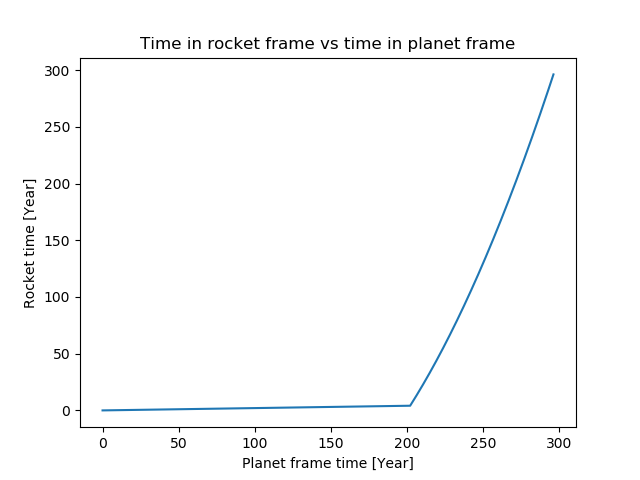
\includegraphics[width=0.8\textwidth]{part8_n.png}
	\caption{The time at P1 in both the spaceship and planet frame.}
	\label{fig:time}
\end{figure}
\FloatBarrier

The code for the plot is:
\lstinputlisting{del8.py}

\item We now want to find the total amount of time that passes in the planet frames clocks during the acceleration phase, as seen from the spaceship frame. Assuming that the spaceship continues with constant acceleration $g$, we have in the first tasks shown that it takes the same amount of time to reach velocity $v=-v_{0}$ and the spaceship will then be at P2 again. In other words, we can use a symmetry argument to find the time that passes in the planet frame before the spaceship reaches P2 again. 
\\
Above we found that when $T_{Y}=\Delta T$ we would have $t_{Y}=t_{Y^{\prime}}\approx296\,\text{years}$. It is now important to remember that the spaceship uses 4 years to reach P2 in the planet frame (as seen from an observer at P1 in the outgoing elevator frame). Hence the time in the planet frame used to accelerate to velocity $v=0$ is \[t_{Y^{\prime}}-t_{B^{\prime}}\approx296\,\text{years}-4\,\text{years}=292\,\text{years}\]
Becasue of our symmetry argument we know that it takes twice the amount of time before the spaceship reaches P2 yet again. This means that the time in the planet frame (as seen from an observer in the returning elevator frame at P1) will be \[t_{\text{Back at P2}}=2\cdot(t_{Y^{\prime}}-t_{B^{\prime}})+t_{B^{\prime}}\approx2\cdot292\,\text{years}+4\,\text{years}=588\,\text{years}\]


\item Now comes the exiting part. We want to calculate how much the astronaut ages during the acceleration phase. We let $(x,t)$ and $(x^{\prime},t^{\prime})$ denote the planet frame and the returning spaceship frame respectively. To make the calculations easier we define event E:

\begin{enumerate} %\begin{itemize}
\item Event E is the spaceship reaching velocity $v=0$ somewhere past P2. Since $v=0$ we must have $t_{E}=t_{E}^{\prime}$, and since the spaceship is always at the origin of its own frame of referance, we must have $x_{E}^{\prime}=0$.
\end{enumerate} %\end{itemize}

We think of the acceleration phase as the astronaut jumping from elevator to elevator, where each elevator has a constant velocity $v_{i}$ for $i=1,2\ldots,n$ and $0=v_{1}<v_{2}<\ldots<v_{i}<v_{i+1}<\ldots<v_{n}=v_{0}$ (note that we now have defined positiv velocity towards P1). The astronaut stays in each elevator a short time interval $\Delta t^{\prime}$. 
\\ \\
We are now ready to find an expression for $\Delta t^{\prime}$. Since each elevator has constant velocity $v_{i}$, the formula for time dilation is still valid. That is, 
\[\Delta t^{\prime}=\Delta t/\gamma=\Delta t\sqrt{1-v_{i}^{2}}\]

So what is $v_{i}$? That depends on which elevator we are in. We will therefore begin thinking of it as only one elevator. As we want to let $\Delta t$ approch zero, we assume that the astronaut had constant acceleration $g$ before he jump on \textquote{this} elevator (the one with velocity $v_{i}$). Hence, by the definition of constant acceleration \ref{eq:def_acc}, the velocity of the elevator is \[v_{i}=gt,\] where $t$ is the time between event E and the astronaut reaching the elevator.
\\
Putting everything together, we find that $\Delta t^{\prime}=\Delta t\sqrt{1-g^{2}t^{2}}$. Assuming that $\Delta t$ is \textquote{small enough} we find that for an arbitrary time interval $\Delta t^{\prime}$ after event E, and an arbitrary elevator with velocity $v_{i}$, we will have \begin{equation}\label{eq:new_time}\Delta t^{\prime}\approx\Delta t\sqrt{1-g^{2}t^{2}}\end{equation}
(We have to let $\Delta t$ be \textquote{small enough}, meaning that the time the astronaut spends in one elevator is so little that we will only have a very small error calculating $\Delta t^{\prime}$)


\item Finally we shall calculate how much the astronaut ages during the acceleration phase. We will do this by calculating the time $t^{\prime}$ in the spaceship frame from event E to the astronaut reaches P2 again. Since we have a symmetric case we know that we can multipy this by two to get our answer.
\\
We start by dividing equation \ref{eq:new_time} by $\Delta t$ and taking the limit as $\Delta t$ approches zero. Since $\Delta t^{\prime}\leq\Delta t$ (see equation for time dilation \ref{eq:time_dila}) we must have $\lim_{\Delta t\to0}\frac{\Delta t^{\prime}}{\Delta t}\geq0$. Thinking of $\Delta t^{\prime}$ as a function of $t$ we therefore get

\[\lim_{\Delta t\to0}\frac{\Delta t^{\prime}}{\Delta t}=\lim_{\Delta t\to0}\sqrt{1-g^{2}t^{2}}\Rightarrow\frac{dt^{\prime}}{dt}=\sqrt{1-g^{2}t^{2}}\]

We can now integrate both sides with respect to the time $dt$. We also need the integration limits. The lower limit must be zero since we want the time from event E to the astronaut reaches P2. In the begining of part 5 we found that the astronaut use $\Delta T=-v_{0}/g$ time to reach velocity $v=0$. The astronaut is now returning to P2, hence the spaceships velocity changes sign. Another way to look at it is that we change which direction is positive. Thus the astronaut use $\Delta T=v_{0}/g=\frac{0.99}{0.1/c}\,s$ to reach P2 (we have now changed the positive direction and therefore also the signs of $v_{0}$ and $g$). That is, the integration limits must be $0$ and $v_{0}/g$. % (remember that we found the time it takes the spaceship to reach velocity $v=0$ when accelerating in the first tasks of part 5, and that we are looking at the symmetric case). 
We therefore have

\begin{align}\label{eq:t_prim}
\frac{dt^{\prime}}{dt}&=\sqrt{1-g^{2}t^{2}} \nonumber\\
\int\frac{dt^{\prime}}{dt}\,dt&=\int\sqrt{1-g^{2}t^{2}}\,dt \nonumber\\
t^{\prime}&=\int_{0}^{-v_{0}/g}\sqrt{1-g^{2}t^{2}}\,dt
\end{align}


\item The easiest way to integrate equation \ref{eq:t_prim} would perhaps be to use an integrator, but we will do it by hand.
\\
To make the integration easier to read, %and hopefully more readable 
we begin by introducing all the formulas and substitutions we need.
\\ \\
\underline{Trigonometric identities:}
\begin{align*}
\cos{2x}&=\cos^{2}{x}-\sin^{2}{x}=\cos^{2}{x}-(1-\cos^{2}{x}) & \sin{2x}&=2\sin{x}\cos{x}\\
\cos^{2}{x}&=\frac{1}{2}(\cos{2x}+1) & \frac{1}{2}\sin{2x}&=\sin{x}\cos{x}
\end{align*}

\underline{Formula for $\cos{\sin^{-1}{u}}$:}
\begin{equation*}
\cos{\sin^{-1}{u}}=\sqrt{1-(\sin{\sin^{-1}{u}})^{2}}=\sqrt{1-u^{2}}
\end{equation*}

\underline{Necessary substitutions:}
\begin{align*}
u^{2}&=g^{2}t^{2} & \frac{dt}{du}&=1/g  &&&  u&=\sin{x} & \frac{du}{dx}&=\cos{x}\\
t&=\frac{u}{g} & \frac{du}{dt}&=g     &&& x&=\sin^{-1}{u} & \frac{dx}{du}&=\frac{1}{\sqrt{1-x^{2}}}
\end{align*}

We are now ready to integrate. We will first find the indefinite integral, change back to our own variables and finally calculate the definite integral. 

\begin{align*}
\int\sqrt{1-g^{2}t^{2}}\,dt&=\frac{1}{g}\int\sqrt{1-u^{2}}\,du=\frac{1}{g}\int\sqrt{1-\sin^{2}{x}}\cos{x}\,dx\\
&=\frac{1}{g}\int\cos^{2}{x}\,dx=\frac{1}{2g}\int\cos{2x}+1\,dx\\
&=\frac{1}{2g}\left(\frac{1}{2}\sin{2x}+x\right)+C=\frac{1}{2g}\left(\cos{x}\sin{x}+x\right)+C\\
&=\frac{1}{2g}\left((\cos{\sin^{-1}{u}})\cdot(\sin{\sin^{-1}{u}})+\sin^{-1}{u}\right)+C=\frac{1}{2g}\left(u\cos{\sin^{-1}{u}}+\sin^{-1}{u}\right)+C\\
&=\frac{1}{2g}\left(u\sqrt{1-u^{2}}+\sin^{-1}{u}\right)+C\\
&=\frac{1}{2g}\left(gt\sqrt{1-g^{2}t^{2}}+\sin^{-1}{g^{2}t^{2}}\right)+C
\end{align*}

\begin{align*}
t^{\prime}&=\int_{0}^{v_{0}/g}\sqrt{1-g^{2}t^{2}}\,dt=\frac{1}{2g}\left[gt\sqrt{1-g^{2}t^{2}}+\sin^{-1}{g^{2}t^{2}}\right]_{0}^{v_{0}/g}\\
&=\frac{1}{2g}\left[g\frac{v_{0}}{g}\sqrt{1-g^{2}\left(\frac{v_{0}}{g}\right)^{2}}+\sin^{-1}\left({g^{2}\left(\frac{v_{0}}{g}\right)^{2}}\right)-g\cdot0\cdot\sqrt{1-g^{2}\cdot0^{2}}-\overbrace{\sin^{-1}\left({g^{2}\cdot0^{2}}\right)}^{=0}\right]\\
&=\frac{1}{2g}\left[v_{0}\sqrt{1-v_{0}^{2}}+\sin^{-1}{v_{0}^{2}}\right]\\
t^{\prime}&=\frac{v_{0}\sqrt{1-v_{0}^{2}}+\sin^{-1}{v_{0}^{2}}}{2g}
\end{align*}


Inserting number, we get
\[t^{\prime}=\frac{0.99\sqrt{1-0.99^{2}}+\sin^{-1}{0.99^{2}}}{2(1/c)}\approx71.8025\,\text{years}\]

In other words, the time experienced by the astronaut during the acceleration phase was $t_{\text{acc}}^{\prime}\approx2\cdot72\,\text{years}=144\,\text{years}$. This means that the entire journey by experienced by the astronaut was \[t_{\text{Total}}^{\prime}=t_{\text{acc}}^{\prime}+2\cdot t_{\text{AB}}^{\prime}\approx144\,\text{years}+57\,\text{years}=201\,\text{years}\]


\item In the final two tasks we want to link what we have just found to gravitation. Let $r$ be the distance from event E, meaning that $r=0$ is at event E. We define positive direction towards P2. We want to find an expression for the position $r$ using the acceleration $g$ and the time $t$, and then solve for the time.
\\
From equation \ref{eq:pos_const_acc} we have $x=x_{0}+v_{0}t+\frac{1}{2}at^{2}$. Let the position of event E be $x=0$. If we choose $x=r$ we have $x_{0}=0$, $v_{0}=0$ and $a=g$, and thus
\[r=0+0\cdot t+\frac{1}{2}gt^{2}=\frac{1}{2}gt^{2}\]

If we now solve for the time we get
\[t=\sqrt{\frac{2r}{g}},\]
just as we wanted.
\\
\textbf{14 og 15 slått sammen}
\\

\item As we have found a new expression for the time $t$, we are allowed to insert this into equation \ref{eq:new_time}. This gives us

\begin{equation}\label{eq:new_time_mark}
\Delta t^{\prime}=\Delta t\sqrt{1-g^{2}t^{2}}=\Delta t\sqrt{1-g^{2}\left(\sqrt{\frac{2r}{g}}\right)^{2}}=\Delta t\sqrt{1-2gr}
\end{equation}

We are now able to link this to gravitation. The gravitational pull by an object is given by $g=\frac{GM}{r^{2}}$. Inserting this into the pervious equation \ref{eq:new_time_mark} we find

\begin{equation}\label{eq:time_grav}
\Delta t^{\prime}=\Delta t\sqrt{1-2gr}=\Delta t\sqrt{1-2r\frac{GM}{r^{2}}}=\Delta t\sqrt{1-\frac{2GM}{r}}
\end{equation}

Equation \ref{eq:time_grav} tells us how time moves in different accelerated frames. This will be important when you learn about general relativity.
\\
\textbf{16 og 17 slått sammen}
\\
\end{enumerate}
\end{enumerate}

\end{document}
